\documentclass[12pt]{article}
\usepackage{graphicx} % For including images/logo
\usepackage{geometry} % For custom margins
\usepackage{fancyhdr} % For custom headers/footers
\usepackage{titling}  % For custom title formatting
\usepackage{amsmath}  % For advanced math formatting
\usepackage{amssymb}  % For additional math symbols
\usepackage{enumitem} % For custom enumeration
\usepackage{xcolor}   % For text coloring
\usepackage{circuitikz}
\usepackage{animate}
\usepackage{algorithm}
\usepackage{algpseudocode}
\usepackage{hyperref}
% Set margins
\geometry{a4paper, margin=1in}

% Title, name, and date
\title{\textbf{EE1060 - DETT GROUP QUIZ 2}}
\author{EE24BTECH11053 - S A Aravind Eswar \\ EE24BTECH11026 - Gunda Srihaas \\ EE24BTECH11009 - A Mokshith Kumar Reddy \\ EE24BTECH11022 - Eshan Sharma \\ EE24BTECH11039 - Mandala Ranjith \\ EE24BTECH11012 - Bhavanisankar G S}
\date{\today}

% Add logo to the title
\pretitle{%
    \begin{center}
    
\includegraphics[width=0.5\textwidth]{figs/IITH.png} \\ % Replace with your logo file
    \vspace{1cm} % Adjust spacing as needed
    \LARGE
}
\posttitle{\end{center}}
\begin{document}

% First page with title, name, date, and logo
\maketitle
\thispagestyle{empty} % Remove page number from the first page

\newpage
\tableofcontents
\newpage


\section{\textbf{Question}}

Compute the convolution of a given signal $f(t)$ with a rectangular kernel $h(t)$, analytically. The rectangular kernel
is defined as:
\begin{align}
h(t) =
\begin{cases}
1, & \text{for } -T \leq t \leq T \\
0, & \text{otherwise}
\end{cases} \label{eq:kernelq}
\end{align}
Derive the convolution expression $y(t) = (f * h)(t)$ in terms of known functions, and analyze the system’s behavior
for various values of the kernel duration $T$ and the input signal $f(t)$. Additionally, investigate the following scenarios:\\
(a) Modify the kernel to only consider the part of the kernel for $t > 0$. How does this affect the convolution result? \\
(b) Shift the kernel by a time $t_0$. \\
Analyze how the shift impacts the convolution output and discuss the significance
of this shift in the context of time-delayed systems. \\
You are free to choose the form of the input signal f(t), but make sure it is well-defined and appropriate for
convolution. A step or sinusoidal signal would work well for this analysis.

\section{\textbf{What is convolution ?}}

Convolution is a mathematical operation on two functions, $f$ and $g$, as the integral of the product of the two functions after one is reflected about the y-axis and shifted, i.e., If we are convolving a signal with a kernel, at each time $t$, we are sliding the kernel over the signal and computing how much they overlap. This is useful in various fields of study like finding the system response given the impulse response, signal processing and in probability.\\
Given two functions $f(x)$ and $g(x)$, convolution of the two signals, \\
\begin{align}
	x(t) &= f(t) * g(t) \\
	     &= \int_{-\infty}^{\infty} f(\tau) g(t - \tau) d \tau \label{eq:conv}
\end{align}
Some properties of convolution : \\
\begin{enumerate}
\item \textbf{Commutativity} : 
\begin{align*}
f(t) * g(t) &= g(t) * f(t)
\end{align*}
\item \textbf{Distributivity} :
\begin{align*}
f(t) * [g(t) + h(t)] &= [f(t) * g(t)] + [f(t) * h(t)] 
\end{align*}
\item \textbf{Associativity} :
\begin{align*}
f(t) * [g(t) * h(t)] &= [f(t) * g(t)] * h(t)
\end{align*}
\item \textbf{Time shifting property} :
If we are given $y(t) = x_1 (t) * x_2 (t)$, then
\begin{align*}
	x_1(t) * x_2(t - T) &= y(t - T) \\
	x_1(t - T) * x_2(t) &= y(t - T) \\
	x_1(t - T_1) * x_2(t - T_2) &= y(t - T_1 - T_2)
\end{align*}
\item \textbf{Width property} :
If the duration of signals $f(t)$ and $g(t)$ are $T_1$ and $T_2$ respectively, then the duration of signal convolving $f(t)$ and $g(t)$ is equal to $T_1 + T_2$
\end{enumerate}

\section{Significance of time-shift}
\begin{enumerate}
\item In time-delayed systems, a positive shift ($t_0$) means that the system responds later to changes in the input. This can cause the system to react too slowly, which may lead to oscillations or instabilities in feedback systems, especially if the system relies on feedback loops (like in control systems or biological systems).
\item A negative shift ($t<0$) might result in the system anticipating the input and responding before it occurs. This could cause overreaction or instability if the system is not designed to handle anticipatory behavior.
\item In devices like thermostat, the system may respond to temperature changes with a delay because of the time it takes to heat/cool the room. By shifting of kernel, if the delay becomes too large, then the system might not be able to track the input accurately, leading to instability (or) oscillations.
\item In the context of signal processing, shifting the kernel corresponds to a phase shift in the signal, e.g., in delay filters, the impulse response can be delayed.
\item In biological systems, time delays are common in processes like hormonal responses, neural signals, or metabolic pathways. Shifting the kernel models how these systems react over time. For example, the delayed release of insulin after glucose intake could be modeled using a time-shifted kernel.

\end{enumerate}

% Ranjith's part
\section{Convolution of step function}

For the kernel in \eqref{eq:kernelq}, we shall find the convolution with $f(t) = u(t)$

\subsection{Analytical Convolution}

Since \( u(\tau) = 0 \) for \( \tau < 0 \), the integral becomes:
\[
y(t) = \int_0^{\infty} h(t - \tau) \, d\tau
\]

We determine the overlap of \( h(t - \tau) \) within its support \( [-T, T] \), resulting in:
\[
t - T \le \tau \le t + T
\]

Intersecting this with \( \tau \ge 0 \), the integration limits become:
\[
\max(0, t - T) \le \tau \le t + T
\]

Thus:
\[
y(t) = \int_{\max(0, t - T)}^{t + T} 1 \, d\tau = t + T - \max(0, t - T)
\]

Breaking into cases:
\[
y(t) =
\begin{cases}
0, & t < -T \\
t + T, & -T \le t < T \\
2T, & t \ge T
\end{cases}
\]

\subsection{Scenario Analysis}

\subsubsection{Causal Kernel}
Modified kernel:
\[
h(t) =
\begin{cases}
1, & 0 \le t \le T \\
0, & \text{otherwise}
\end{cases}
\]

Now:
\[
y(t) = \int_0^\infty h(t - \tau) \, d\tau
= \int_{\max(0, t - T)}^{t} 1 \, d\tau = \min(t, T)
\]

Thus:
\[
y(t) =
\begin{cases}
0, & t < 0 \\
t, & 0 \le t < T \\
T, & t \ge T
\end{cases}
\]

\subsubsection{Shifted Kernel}
Let \( h(t) \rightarrow h(t - \tau_0) \). Then:
\[
y(t) = \int_0^\infty u(\tau) h(t - \tau - \tau_0) \, d\tau = y_{\text{original}}(t - \tau_0)
\]

The output is simply delayed by \( \tau_0 \).

The corresponding graphs are shown below - \\
\begin{figure}[h]
    \centering
    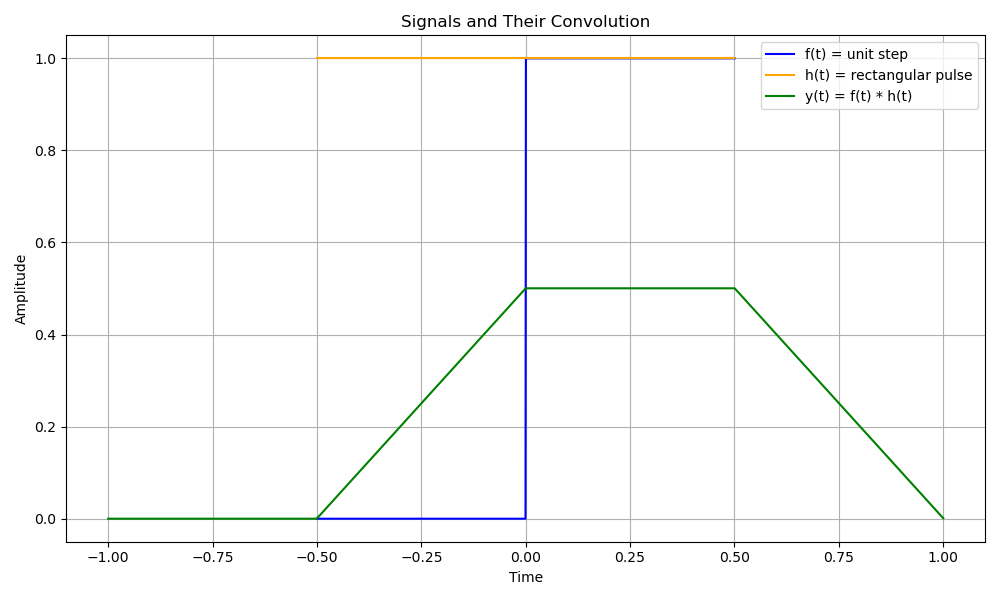
\includegraphics[width=0.6\textwidth]{figs/t_0.5.png}
    \caption{T = 0.5}
    \label{fig:t_0.5.png}
\end{figure}
\begin{figure}[h]
    \centering
    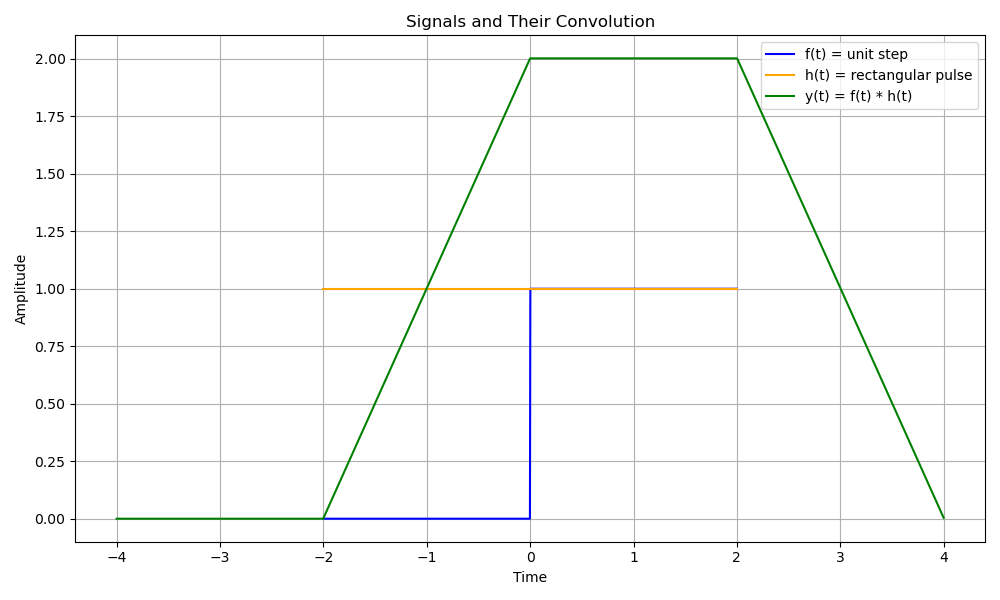
\includegraphics[width=0.6\textwidth]{figs/t_2.png}
    \caption{T = 2}
    \label{fig:conv_sinc}
\end{figure}
\begin{figure}[h]
    \centering
    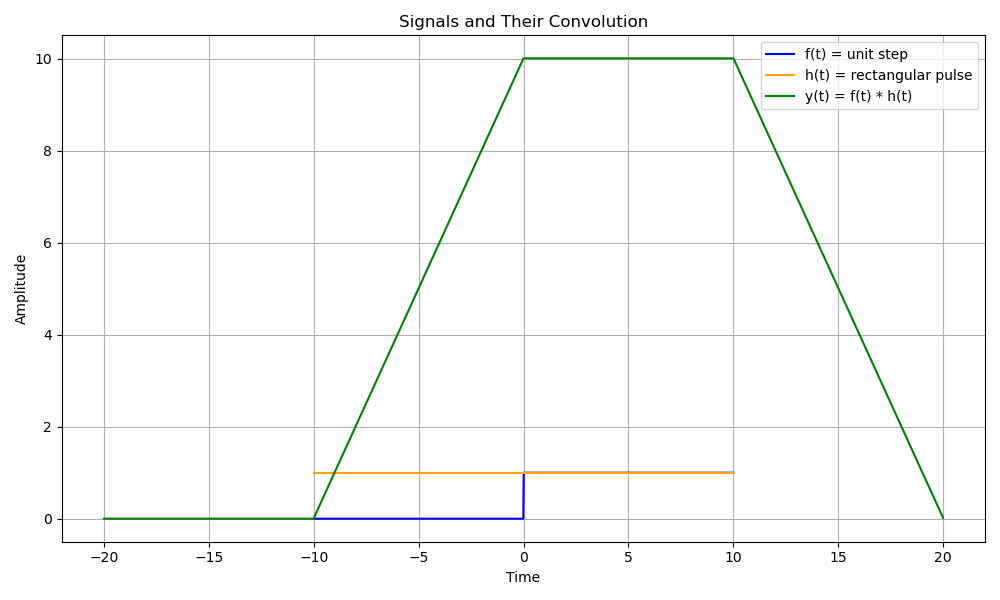
\includegraphics[width=0.6\textwidth]{figs/t_10.png}
    \caption{T = 10}
    \label{fig:conv_sinc}
\end{figure}

\newpage

\documentclass{article}
\usepackage{graphicx}
\usepackage{amsmath,amssymb,amsthm}
\usepackage{float}
\usepackage{array}


\title{Convolution}
\author{Gunda Srihaas}
\date{}

\begin{document}

\maketitle

\section{Question} 
Compute the convolution of a given signal f(t) with a rectangular kernel h(t), analytically. The rectangular kernel
is defined as:
\[
h(t)=
\begin{cases}
    1, & \text{for } -T \leq t \leq T \\
    0, & \text{otherwise}
\end{cases}
\]
Derive the convolution expression $y(t) = (f * h)(t)$ in terms of known functions, and analyze the system’s behavior
for various values of the kernel duration T and the input signal $f(t)$. Additionally, investigate the following scenarios:\\
\begin{enumerate}
\item[a.] Modify the kernel to only consider the part of the kernel for $t > 0$. How does this affect the convolution result?\\
\item [b.] Shift the kernel by a time $\tau_0$. Analyze how the shift impacts the convolution output and discuss the significance
of this shift in the context of time-delayed systems
\end{enumerate}

\section{Solution}
\subsection{\textbf{Taking $f(t)= sin(\omega t)$}}
The convolution is defined as:
\begin{align*}
y(t) = (f * h)(t) = \int_{-\infty}^{\infty} f(\tau) h(t - \tau) \, d\tau
\end{align*}

Given,
\begin{align*}
h(t)=
\begin{cases}
    1, & \text{for } -T \leq t \leq T \\
    0, & \text{otherwise}
\end{cases}
\end{align*}

Which implies in convolution,
\begin{align*}
    -T \leq t - \tau \leq T \\
    t-T \leq \tau \leq t+T
\end{align*}

$\implies h(t-\tau)=1$ in $(t-T,t+T)$
\\
Thus, the convolution integral becomes:
\begin{align*}
y(t) = \int_{t - T}^{t + T} f(\tau) \, d\tau
\end{align*}

For $f(t) = \sin(\omega t)$, the convolution becomes:
\[
y(t) = \int_{t - T}^{t + T} \sin(\omega \tau) \, d\tau
\]

\begin{align*}
y(t) &= \int_{t - T}^{t + T} \sin(\omega \tau) \, d\tau \\
&= \left[ -\frac{1}{\omega} \cos(\omega \tau) \right]_{t - T}^{t + T} \\
&= -\frac{1}{\omega} \left[ \cos(\omega (t + T)) - \cos(\omega (t - T)) \right]
\end{align*}

Using the trigonometric identity:
\begin{align*}
\cos A - \cos B = -2 \sin\left(\frac{A + B}{2}\right) \sin\left(\frac{A - B}{2}\right) \end{align*}

Let:
\begin{align*}
A &= \omega (t + T) \\
B &= \omega (t - T)
\end{align*}

Then:
\begin{align*}
\frac{A + B}{2} &= \omega t \\
\frac{A - B}{2} &= \omega T
\end{align*}

Substituting:
\begin{align*}
y(t) &= -\frac{1}{\omega} \left[ -2 \sin(\omega t) \sin(\omega T) \right] \\
&= \frac{2}{\omega} \sin(\omega T) \sin(\omega t)
\end{align*}

\textbf{Final Result}
\begin{align*}
y(t) = \frac{2}{\omega} \sin(\omega T) \sin(\omega t)    
\end{align*}
\newpage
\subsection{Taking any periodic $f(t)$}
\begin{align*}
f(t) = A_0 + \sum_{n=1}^\infty A_n \cos\left(\frac{n\pi t}{L}\right) + \sum_{n=1}^\infty B_n \sin\left(\frac{n\pi t}{L}\right)
\end{align*}
By substitution of $f(t)$ and and reducing the integral we get
\begin{align*}
y(t) = \int_{t - T/2}^{t + T/2} \left[ A_0 + \sum_{n=1}^\infty A_n \cos\left(\frac{n\pi \tau}{L}\right) + \sum_{n=1}^\infty B_n \sin\left(\frac{n\pi \tau}{L}\right) \right] d\tau
\end{align*}
\\
\textbf{DC Term}
\begin{align*}
\int_{t - T/2}^{t + T/2} A_0 \, d\tau = A_0 T
\end{align*}
\\
\paragraph{Sine part}
\begin{align*}
B_n \int \sin\left(\frac{n\pi \tau}{L}\right) d\tau = -\frac{L}{n\pi} \cos\left(\frac{n\pi \tau}{L}\right)
\end{align*}
Evaluating from $t - T/2$ to $t + T/2$:
\begin{align*}
B_n \cdot \frac{2L}{n\pi} \cos\left(\frac{n\pi t}{L}\right) \sin\left(\frac{n\pi T}{2L}\right)
\end{align*}
\\
\textbf{Cosine part}
\begin{align*}
y_{\text{cos}}(t) &= \int_{t - T}^{t + T} A_n \cos\left(\frac{n\pi \tau}{L}\right) \, d\tau \\
&= A_n \left[ \frac{L}{n\pi} \sin\left(\frac{n\pi \tau}{L}\right) \right]_{t - T}^{t + T} \\
&= A_n \cdot \frac{L}{n\pi} \left[ \sin\left(\frac{n\pi (t + T)}{L}\right) - \sin\left(\frac{n\pi (t - T)}{L}\right) \right]
\end{align*}

Using the trigonometric identity:
\begin{align*}
\sin C - \sin D = 2 \cos\left(\frac{C + D}{2}\right) \sin\left(\frac{C - D}{2}\right)
\end{align*}

Let:
\begin{align*}
C &= \frac{n\pi (t + T)}{L} = \frac{n\pi t}{L} + \frac{n\pi T}{L} \\
D &= \frac{n\pi (t - T)}{L} = \frac{n\pi t}{L} - \frac{n\pi T}{L}
\end{align*}

Then:
\begin{align*}
\frac{C + D}{2} &= \frac{n\pi t}{L} \\
\frac{C - D}{2} &= \frac{n\pi T}{L}
\end{align*}

Substituting:
\begin{align*}
y_{\text{cos}}(t) &= A_n \cdot \frac{L}{n\pi} \left[ 2 \cos\left(\frac{n\pi t}{L}\right) \sin\left(\frac{n\pi T}{L}\right) \right] \\
&= A_n \cdot \frac{2L}{n\pi} \sin\left(\frac{n\pi T}{L}\right) \cos\left(\frac{n\pi t}{L}\right)
\end{align*}

\subsection*{Final Result}
\begin{align*}
y(t) = 2A_0 T + \sum_{n=1}^\infty \frac{2L}{n\pi} \sin\left(\frac{n\pi T}{L}\right) \left[ A_n \sin\left(\frac{n\pi t}{L}\right) + B_n \cos\left(\frac{n\pi t}{L}\right) \right]
\end{align*}

\section*{Convolution of a Signal with a Rectangular Kernel}

Given a signal $f(t)$ and a rectangular kernel $h(t)$ defined as:
\[
h(t)=
\begin{cases}
    1, & \text{for } -T \leq t \leq T \\
    0, & \text{otherwise}
\end{cases}
\]
The convolution $y(t) = (f * h)(t)$ is:
\begin{align*}
y(t) = \int_{-\infty}^{\infty} f(\tau) h(t - \tau) \,d\tau
\end{align*}

\subsection*{Part 1: General Convolution Expression}
The kernel $h(t - \tau)$ is 1 when $-T \leq t - \tau \leq T$, i.e., $t - T \leq \tau \leq t + T$. Thus:
\begin{align*}
y(t) = \int_{t - T}^{t + T} f(\tau) \,d\tau
\end{align*}

\subsection*{Part 2: Analysis for Various $T$ and $f(t)$}
\begin{itemize}
    \item \textbf{Large $T$:} More smoothing of $f(t)$, attenuates high frequencies.
    \item \textbf{Small $T$:} Less smoothing, $y(t) \approx f(t)$.
    \item \textbf{Constant $f(t) = c$:} $y(t) = 2T c$.
    \item \textbf{Linear $f(t) = a t + b$:} 
    \begin{align*}
    y(t) &= \int_{t - T}^{t + T} (a \tau + b) \,d\tau \\
         &= 2a T t + 2T b
    \end{align*}
\end{itemize}

\subsection*{Part a: Modified Kernel ($t > 0$)}
Define:
\[
h_{\text{modified}}(t)=
\begin{cases}
    1, & \text{for } 0 \leq t \leq T \\
    0, & \text{otherwise}
\end{cases}
\]
The convolution becomes:
\begin{align*}
y_{\text{modified}}(t) = \int_{t - T}^{t} f(\tau) \,d\tau
\end{align*}
\textbf{Difference:}
\begin{itemize}
    \item Original: Integrates symmetrically around $t$ ($[t - T, t + T]$).
    \item Modified: Only integrates past values ($[t - T, t]$), making it causal.
\end{itemize}

\subsection*{Part b: Shifted Kernel by $\tau_0$}
Shifted kernel:
\[
h_{\text{shifted}}(t) = h(t - \tau_0) =
\begin{cases}
    1, & \text{for } \tau_0 - T \leq t \leq \tau_0 + T \\
    0, & \text{otherwise}
\end{cases}
\]
The convolution is:
\begin{align*}
y_{\text{shifted}}(t) &= \int_{t - \tau_0 - T}^{t - \tau_0 + T} f(\tau) \,d\tau \\
                      &= y(t - \tau_0)
\end{align*}
\textbf{Interpretation:} Shifting the kernel by $\tau_0$ shifts the output by $\tau_0$.

\subsection*{Specific Cases for $f(t)$}
\subsubsection*{Case 1: $f(t) = \sin(\omega t)$}
\begin{align*}
y(t) &= \int_{t - T}^{t + T} \sin(\omega \tau) \,d\tau \\
     &= \frac{2 \sin(\omega T)}{\omega} \sin(\omega t)
\end{align*}
For shifted kernel:
\begin{align*}
y_{\text{shifted}}(t) = \frac{2 \sin(\omega T)}{\omega} \sin(\omega (t - \tau_0))
\end{align*}

\subsubsection*{Case 2: Fourier Series Representation}
Let:
\begin{align*}
f(t) = A_0 + \sum_{n=1}^\infty A_n \cos\left(\frac{n\pi t}{L}\right) + \sum_{n=1}^\infty B_n \sin\left(\frac{n\pi t}{L}\right)
\end{align*}
Then:
\begin{align*}
y(t) &= 2 T A_0 + \sum_{n=1}^\infty \frac{2 L}{n \pi} \sin\left(\frac{n \pi T}{L}\right) \left[ A_n \cos\left(\frac{n \pi t}{L}\right) + B_n \sin\left(\frac{n \pi t}{L}\right) \right]
\end{align*}
For shifted kernel:
\begin{align*}
y_{\text{shifted}}(t) &= 2 T A_0 + \sum_{n=1}^\infty \frac{2 L}{n \pi} \sin\left(\frac{n \pi T}{L}\right) \\
&\quad \times \left[ A_n \cos\left(\frac{n \pi (t - \tau_0)}{L}\right) + B_n \sin\left(\frac{n \pi (t - \tau_0)}{L}\right) \right]
\end{align*}

\begin{figure}[H]
    \centering
    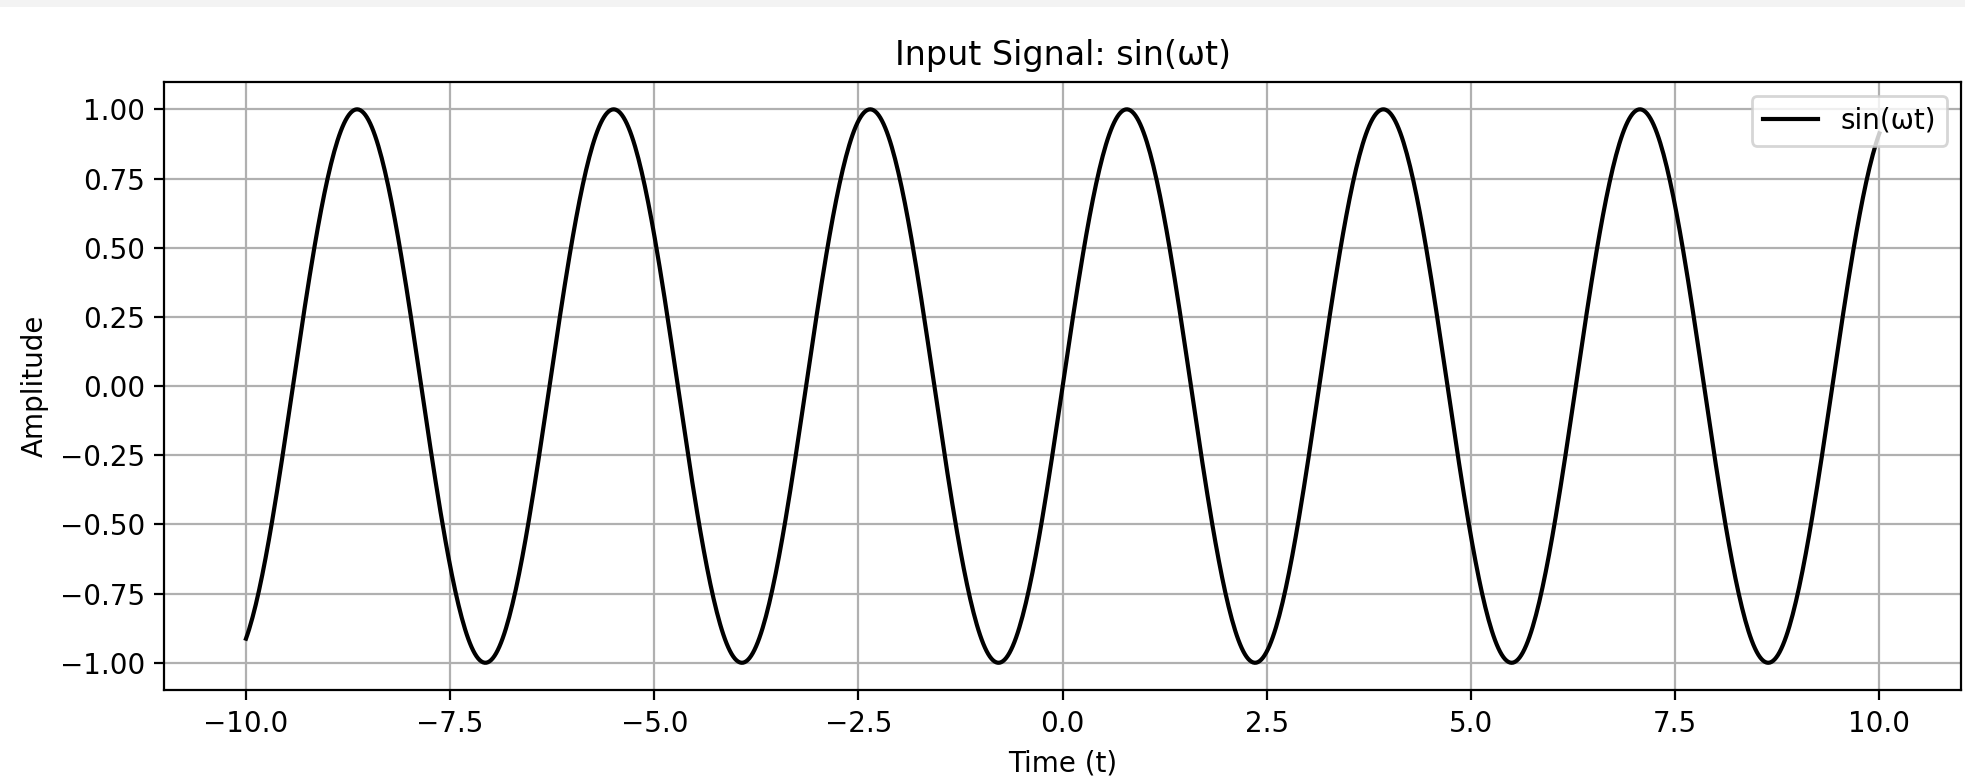
\includegraphics[width=\linewidth]{figs/sinwt.png}
\end{figure}
\begin{figure}[H]
    \centering
    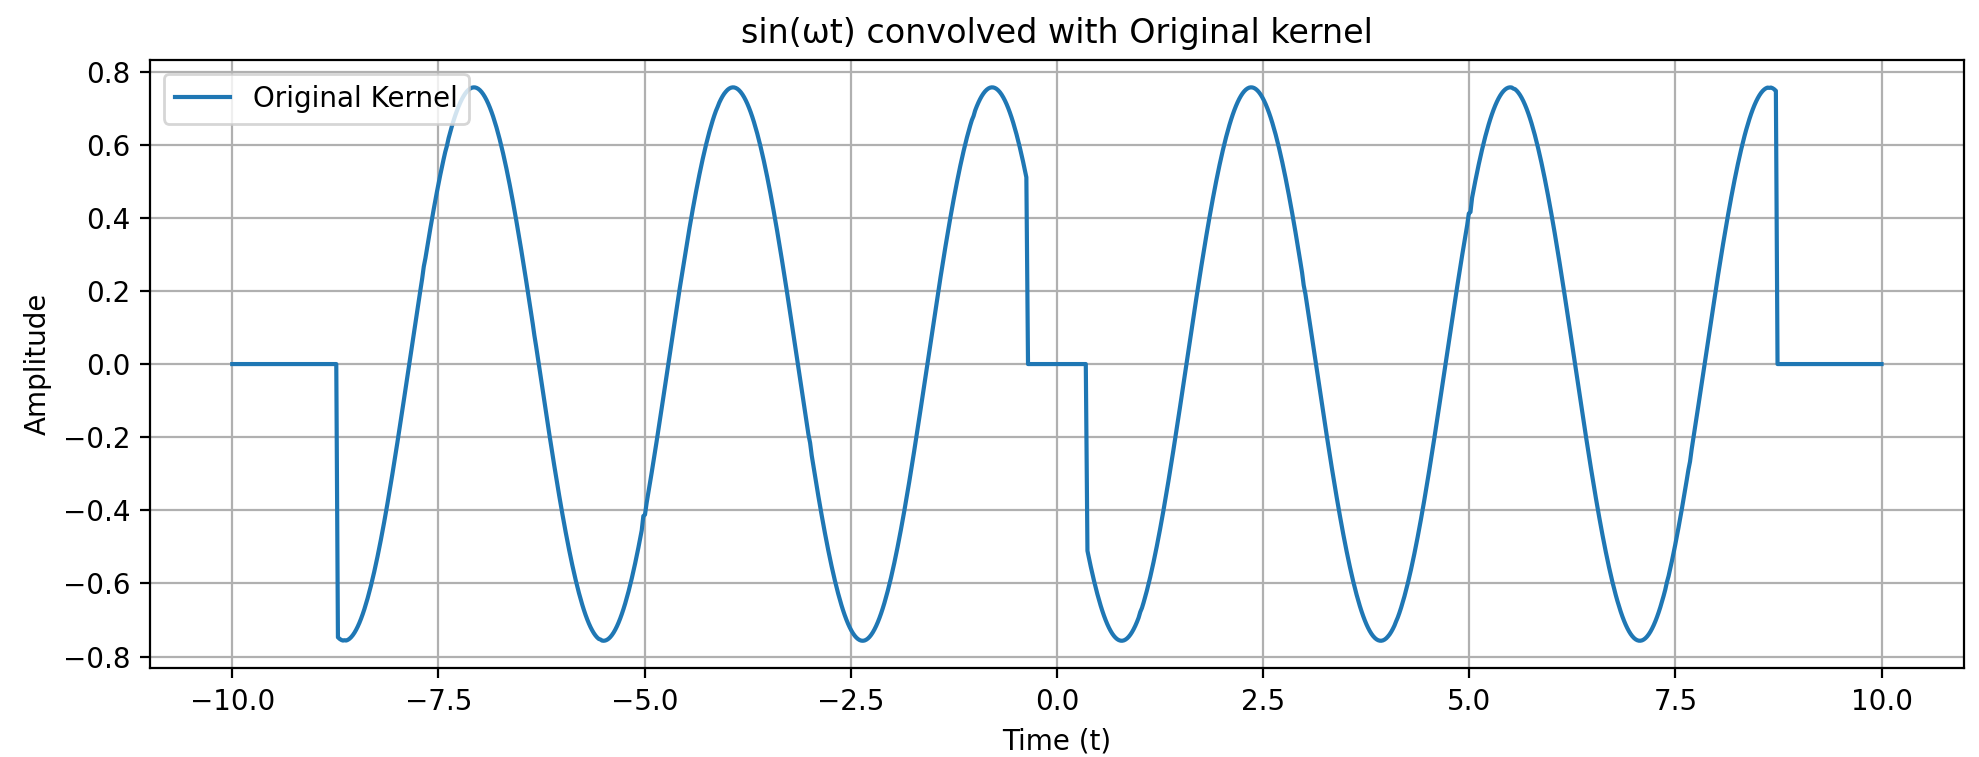
\includegraphics[width=\linewidth]{figs/sinconv.png}
\end{figure}
\newpage
\begin{figure}[H]
    \centering
    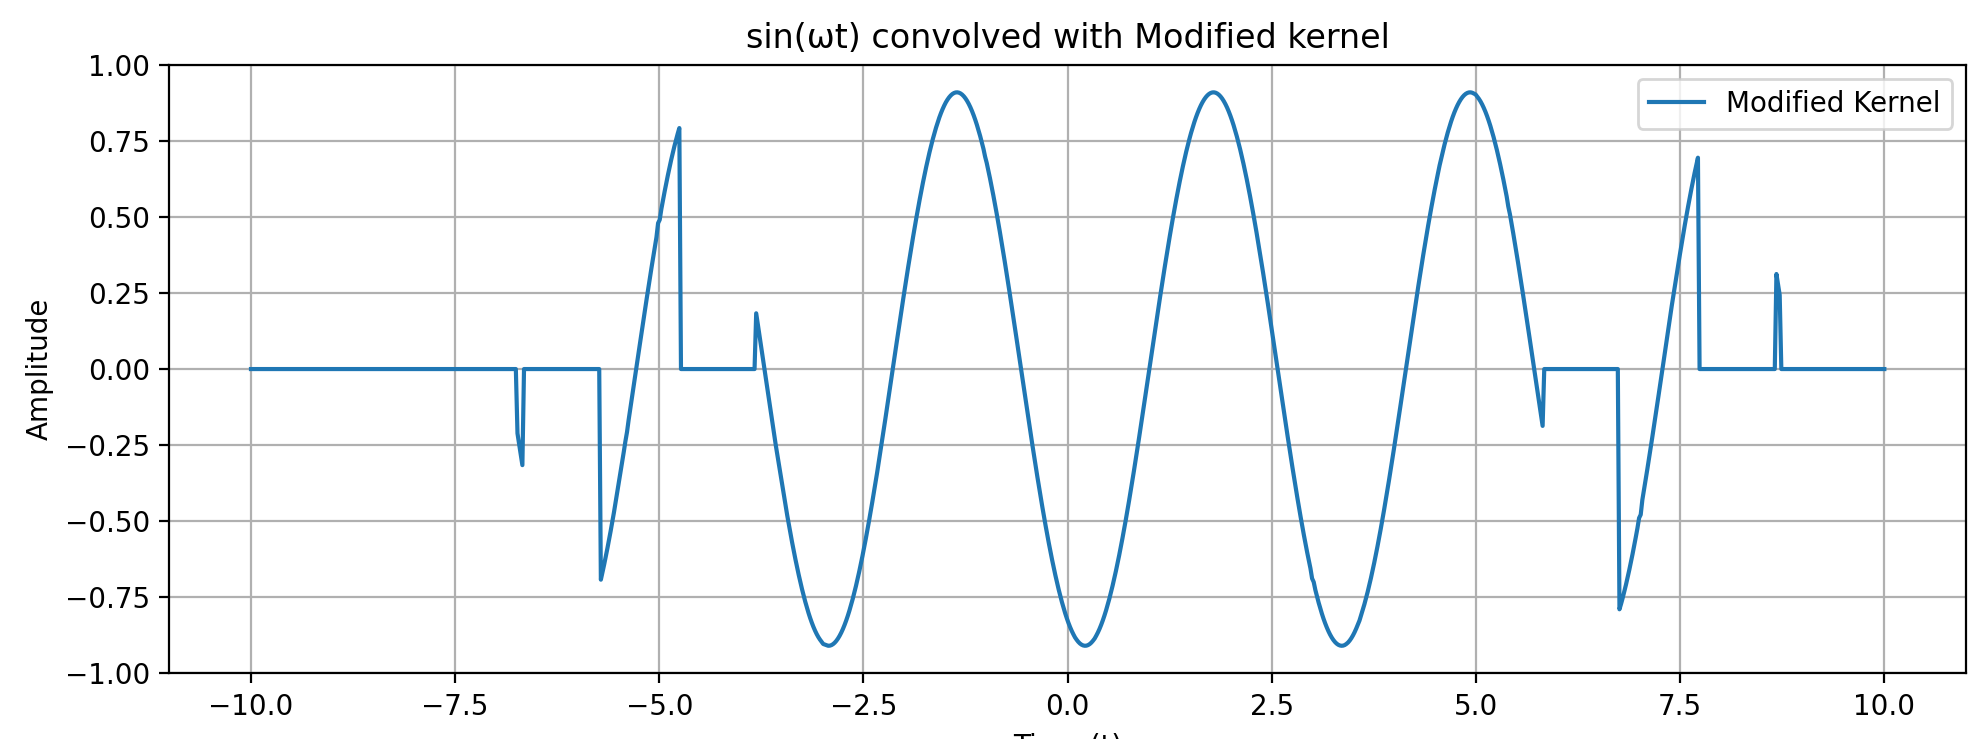
\includegraphics[width=\linewidth]{figs/modifiedsin.png}
\end{figure}
\begin{figure}[H]
    \centering
    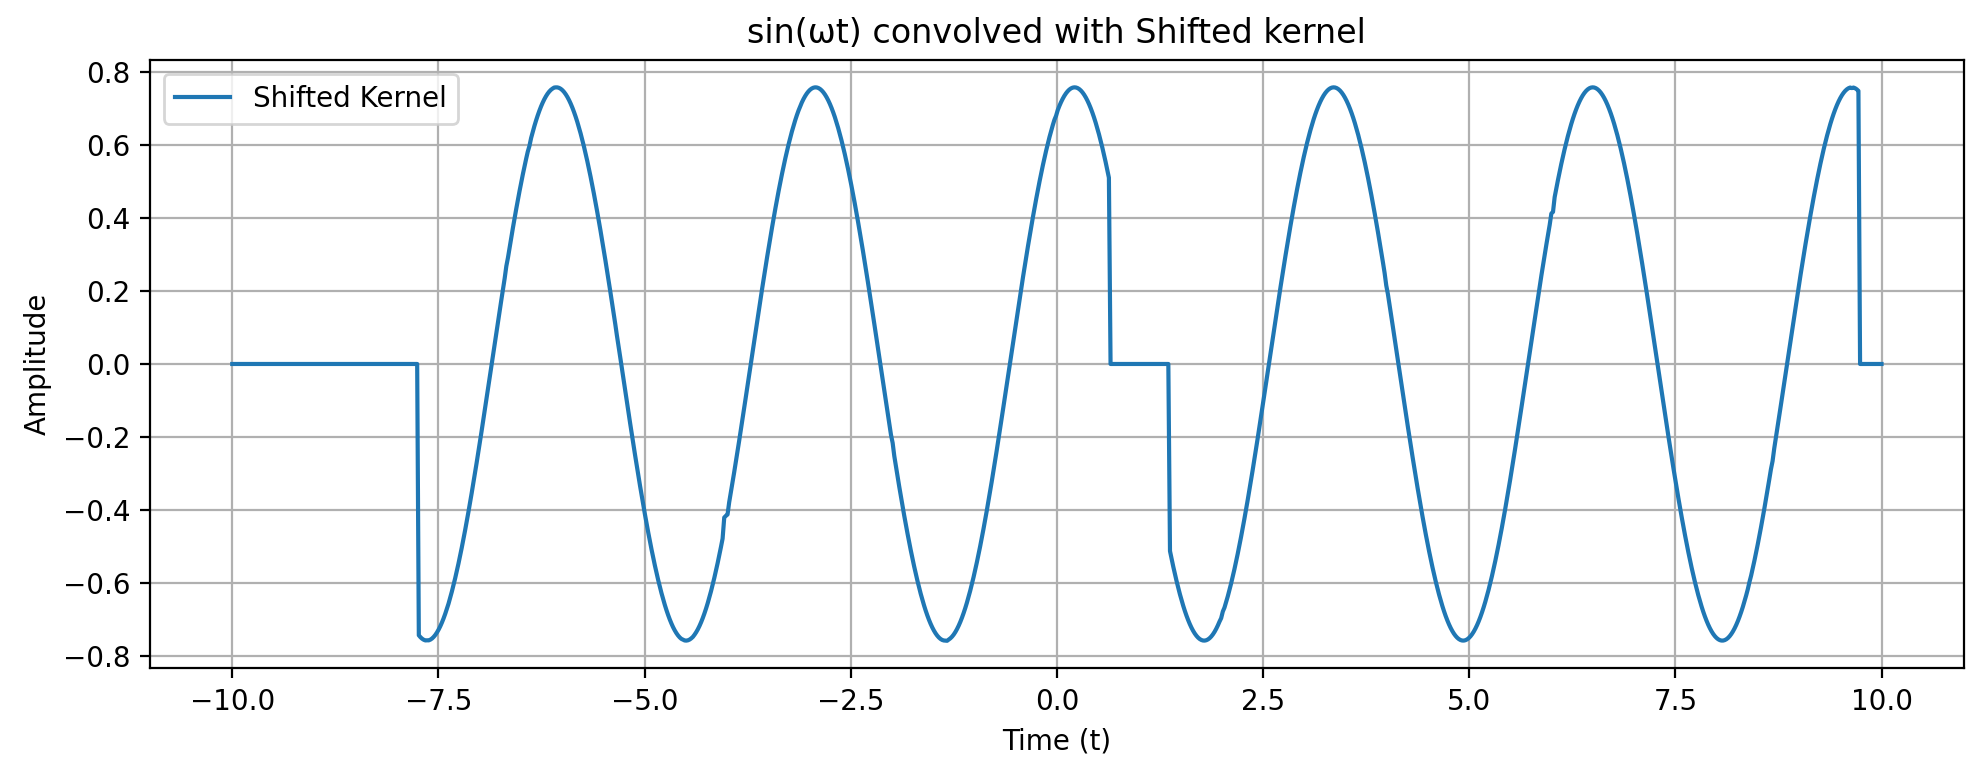
\includegraphics[width=\linewidth]{figs/shiftedsin.png}
\end{figure}

\begin{figure}[H]
    \centering
    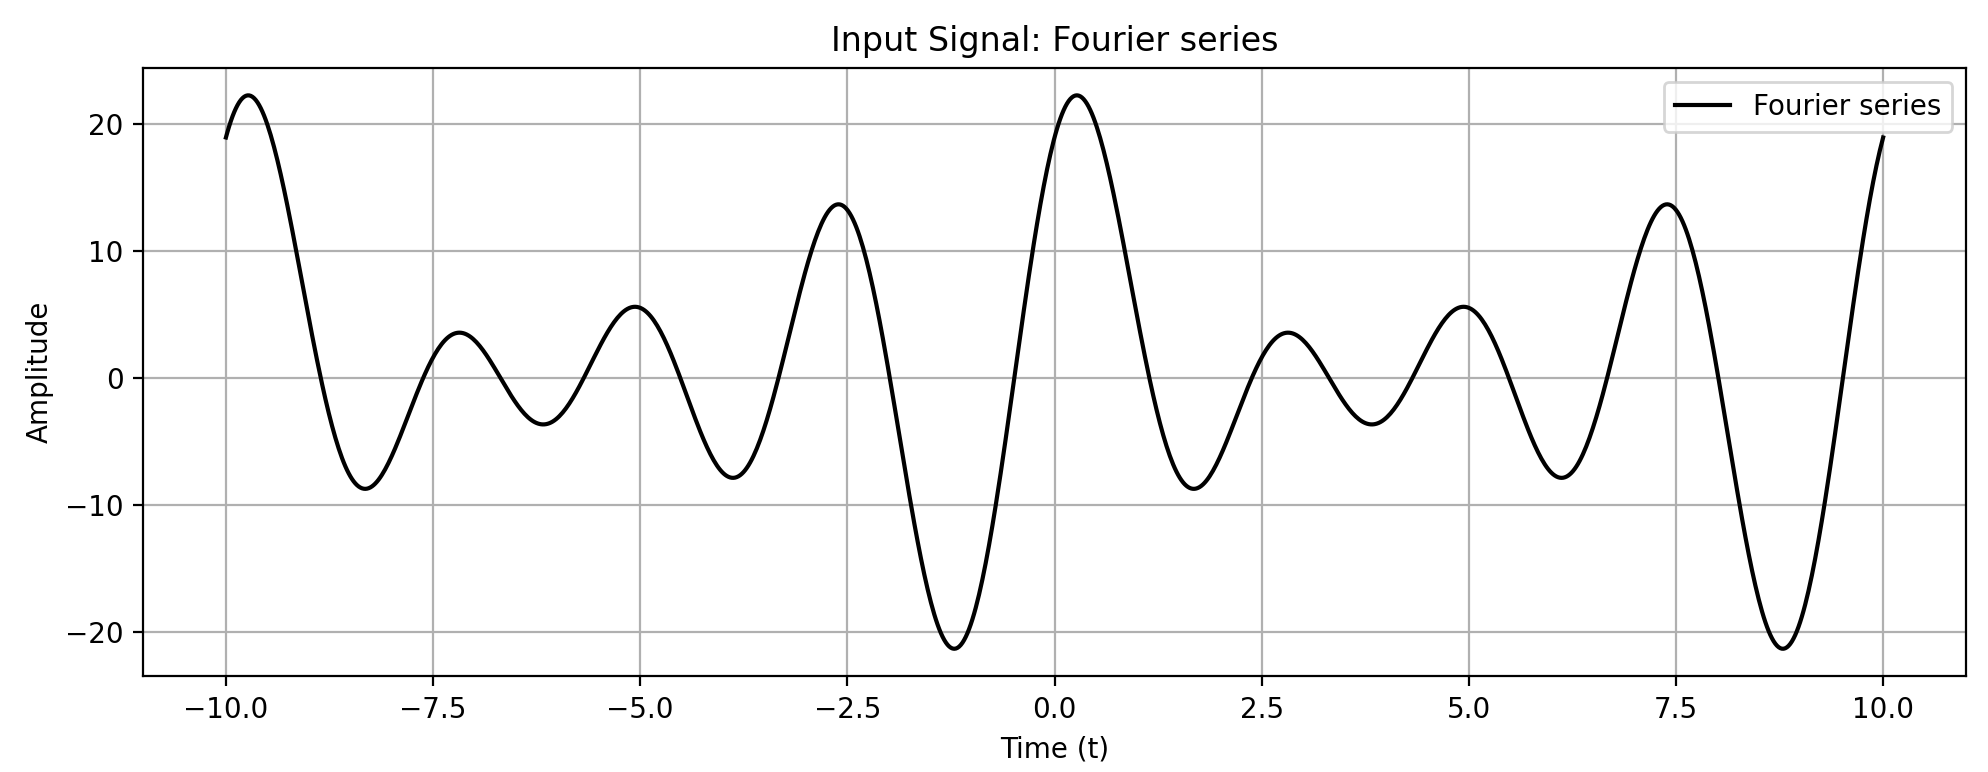
\includegraphics[width=\linewidth]{figs/fourierbreak.png}
\end{figure}
\begin{figure}[H]
    \centering
    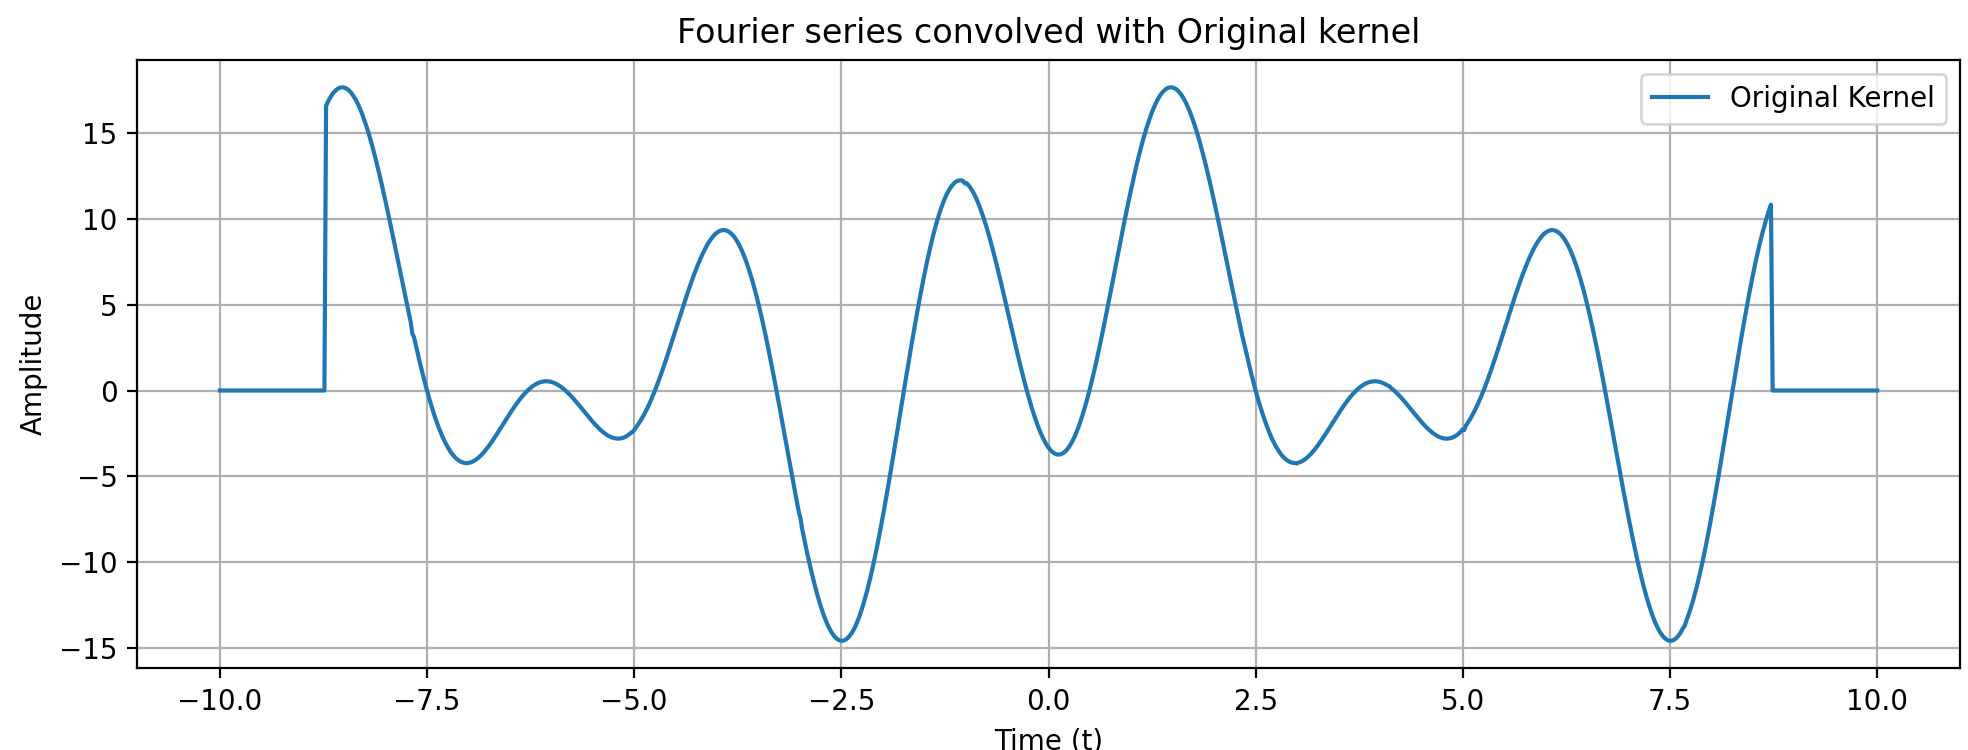
\includegraphics[width=\linewidth]{figs/fourierconv.png}
\end{figure}
\begin{figure}[H]
    \centering
    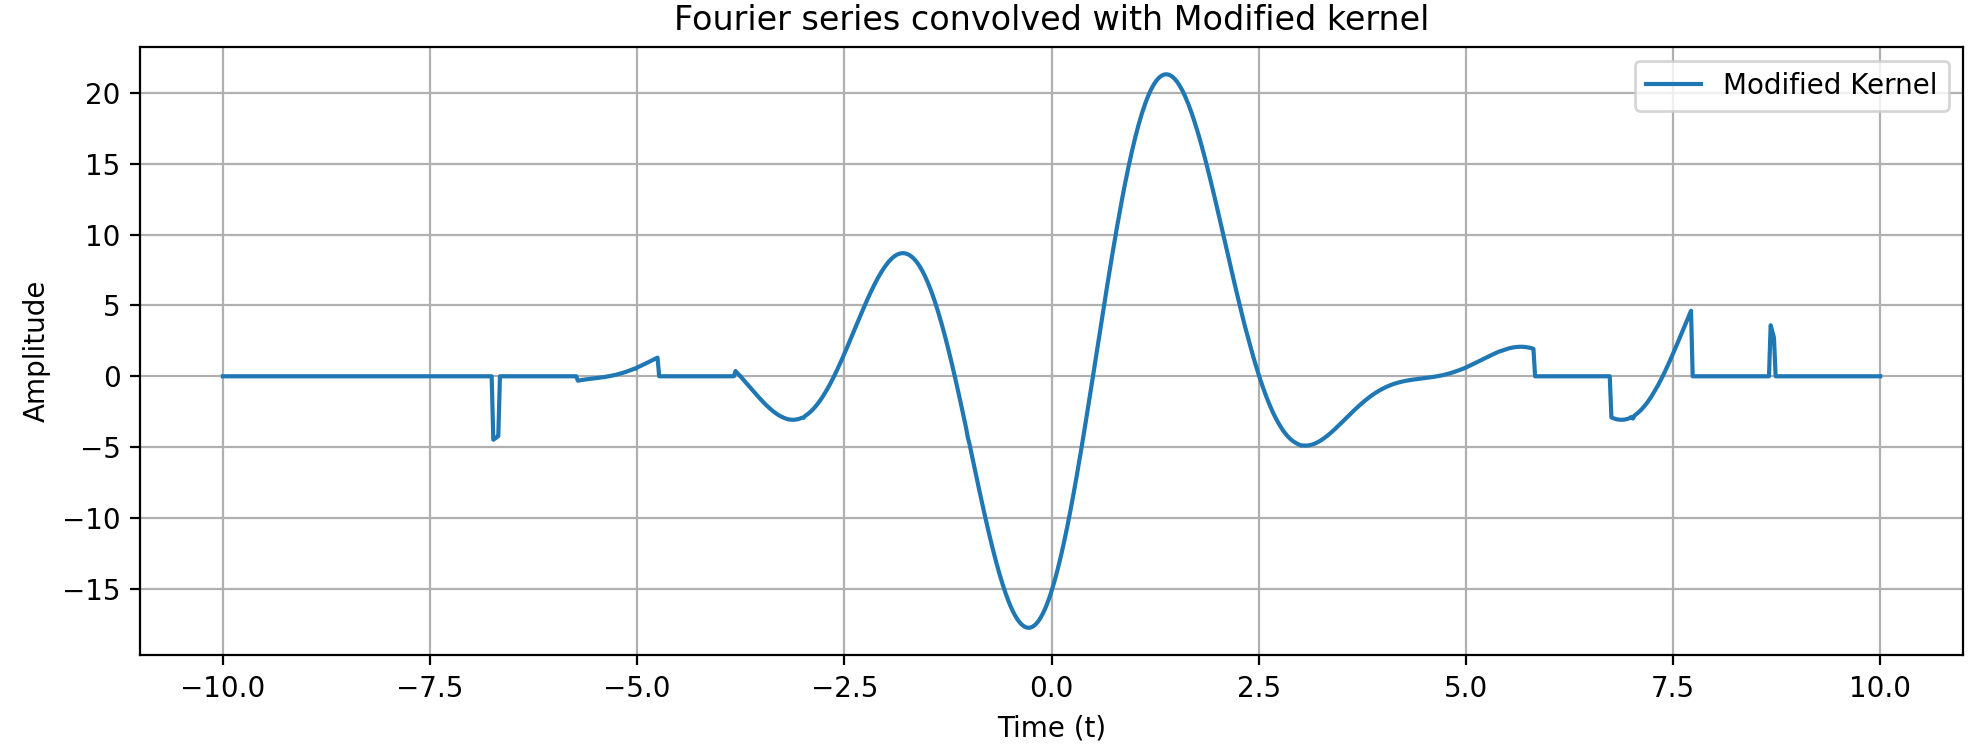
\includegraphics[width=\linewidth]{figs/modifiedfourier.png}
\end{figure}
\begin{figure}[H]
    \centering
    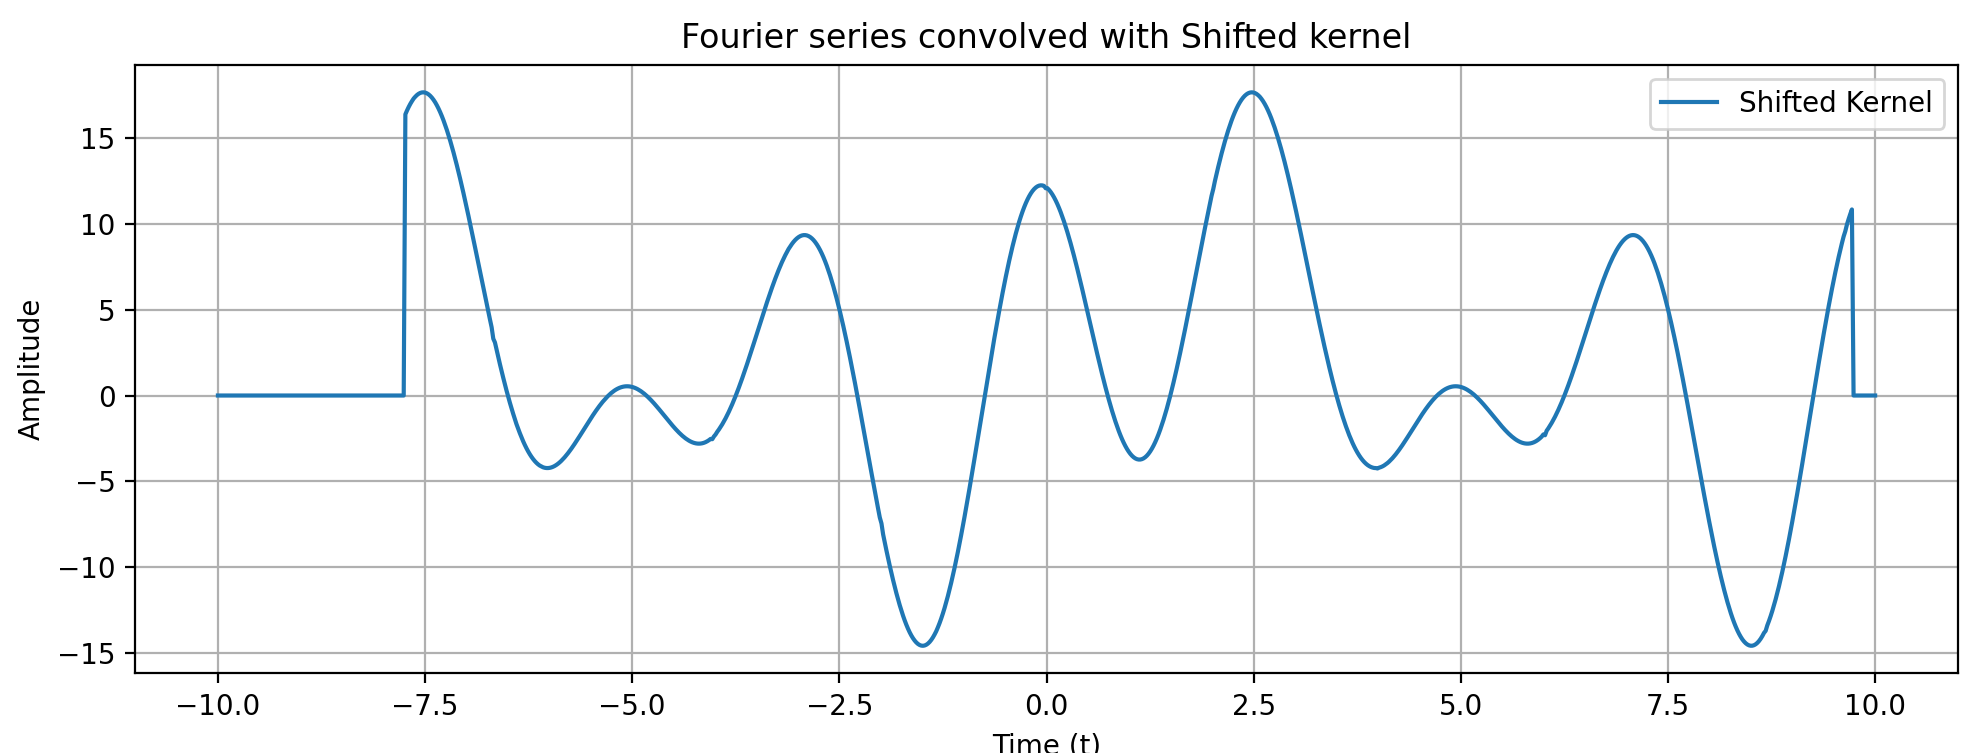
\includegraphics[width=\linewidth]{figs/shiftedfourier.png}
\end{figure}

\end{document}

\section{Convolution of linear function}

Given kernel, 
\[
h(t) =
\begin{cases}
1, & \text{for } -T \leq t \leq T \\
0, & \text{otherwise}
\end{cases}
\]
and the function 
\begin{align*}
f(t) &= at+b
\end{align*}
Let $y(t) = x(t) * f(t)$, then
\begin{align*}
	y(t) &= h(t) * f(t) \\
             &= f(t) * h(t) \\
             &= \int_{-\infty}^{\infty} f(\tau) h(t - \tau) d \tau \\
\end{align*}
\[
h(t - \tau) =
\begin{cases}
1, & \text{for } -T \leq t - \tau \leq T \\
0, & \text{otherwise}
\end{cases}
\]
\[
h(t - \tau) =
\begin{cases}
1, & \text{for } \tau - T \leq t \leq \tau + T \\
0, & \text{otherwise}
\end{cases}
\]
Therefore, the convolution becomes, 
\begin{align*}
	y(t) &= \int_{t - T}^{t + T} (at+b)* 1 d\tau \\
	y(t) &= \int_{t - T}^{t + T}  (at+b)d\tau\\
    y(t) &= \frac{a}{2}[(t+T)^2-(t-T)^2]+b[t+T-(t-T)]\\
    y(t) &= 2atT+2bT
\end{align*}
This integration can be numerically computed and can be seen to be the following - (we are using the values of  and b as 1)\\
\newpage
For different values of T, the change in $y(t)$ is depicted in the following - \\
\begin{figure}[h]
    \centering
    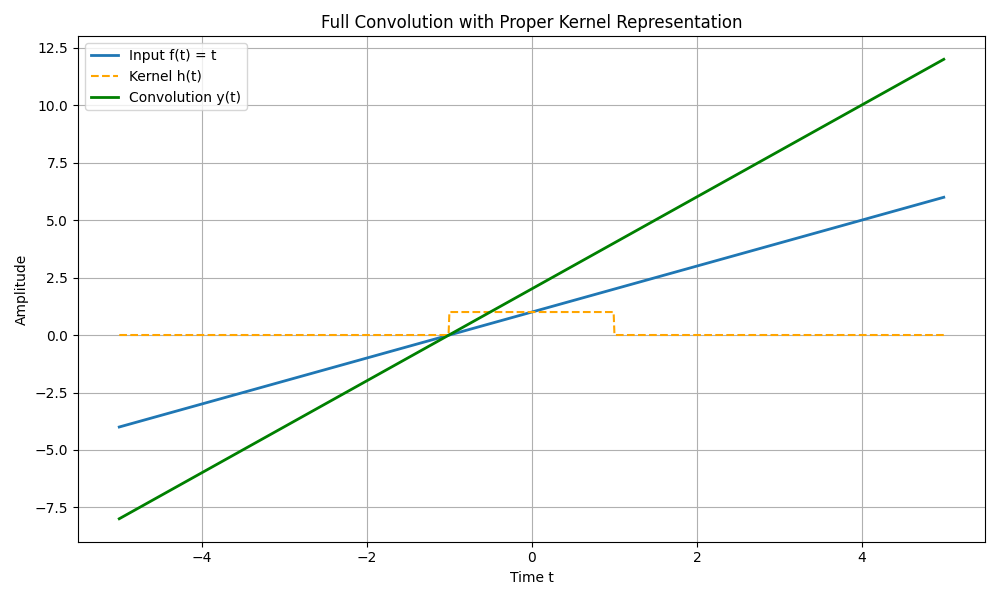
\includegraphics[width=0.6\textwidth]{figsm/1.png}
    \caption{T = 1}
    \label{fig:conv_sinc}
\end{figure}
\begin{figure}[h]
    \centering
    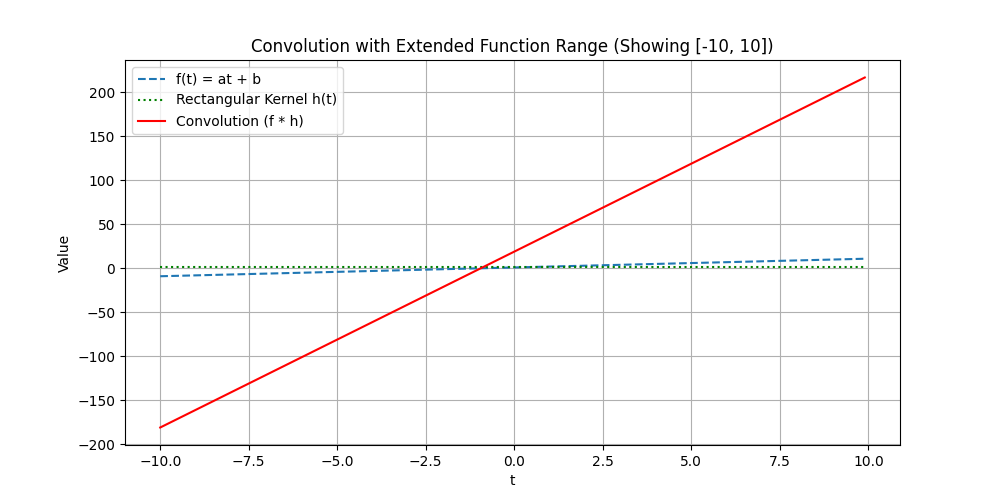
\includegraphics[width=0.6\textwidth]{figsm/2.png}
    \caption{T = 1}
    \label{fig:conv_sinc}
\end{figure}
It can be seen that as $T$ increases, the slope of the output is increasing but it is still linear.
\newpage
\subsection{Considering the kernel for $t>0$}
The response of the system for different values of $T$ are as follows -\\
Modified kernel is, 
\[
h(t) =
\begin{cases}
1, & \text{for} 0 \leq t \leq T \\
0, & \text{otherwise}
\end{cases}
\]
and the function 
\begin{align*}
f(t) &= at+b
\end{align*}
Let $y(t) = x(t) * f(t)$, then
\begin{align*}
	y(t) &= h(t) * f(t) \\
             &= f(t) * h(t) \\
             &= \int_{-\infty}^{\infty} f(\tau) h(t - \tau) d \tau \\
\end{align*}
\[
h(t - \tau) =
\begin{cases}
1, & \text{for } 0 \leq t - \tau \leq T \\
0, & \text{otherwise}
\end{cases}
\]
\[
h(t - \tau) =
\begin{cases}
1, & \text{for } \tau - T \leq t \leq \tau \\
0, & \text{otherwise}
\end{cases}
\]
Therefore, the convolution becomes, 
\begin{align*}
	y(t) &= \int_{t - T}^{t + T} (at+b)* 1 d\tau \\
	y(t) &= \int_{t - T}^{t + T}  (at+b)d\tau\\
    y(t) &= \frac{a}{2}[(t)^2-(t-T)^2]+b[t-(t-T)]\\
    y(t) &= atT-\frac{a}{2}{T}^2+bT
\end{align*}
\begin{figure}[h]
    \centering
    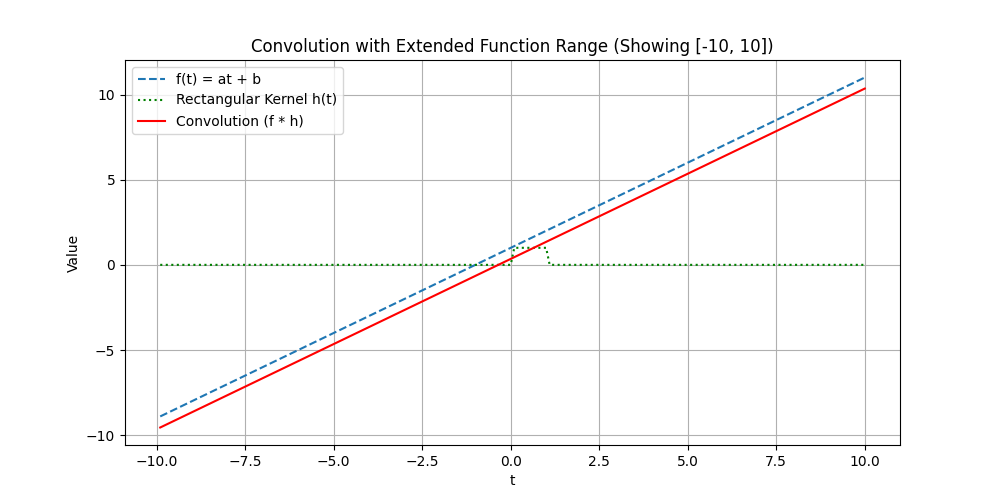
\includegraphics[width=0.6\textwidth]{figsm/3.png}
    \caption{T = 1,A=1,B=1}
    \label{fig:conv_sinc}
\end{figure}
\begin{figure}[h]
    \centering
    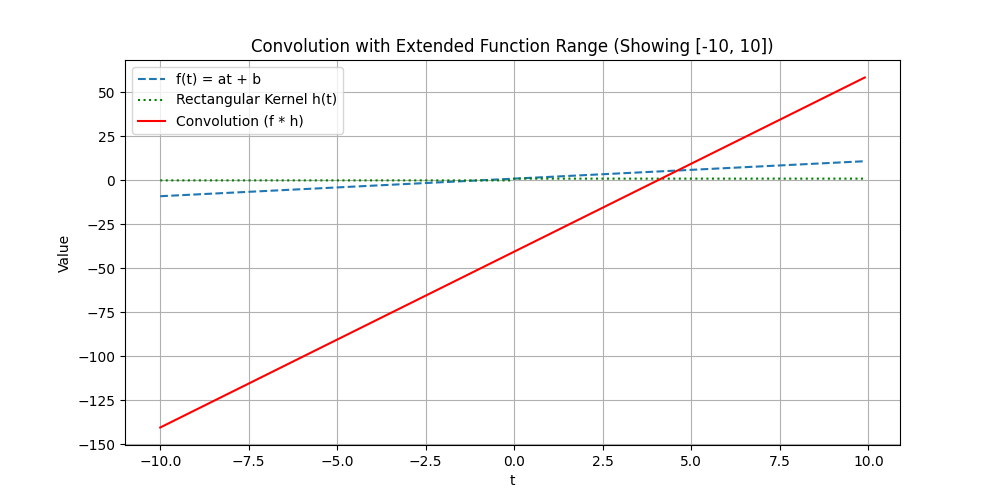
\includegraphics[width=0.6\textwidth]{figsm/4.png}
    \caption{T = 10,A=1,B=1}
    \label{fig:conv_sinc}
\end{figure}
\newpage

\subsection{Shifting the kernel by $t_{0}$}
Shifting of kernel means moving the kernel to the left or right by an amount, i.e., if the given kernel is shifted by an amount $t_0$, then it becomes, 
\[
h(t) =
\begin{cases}
1, & \text{for } -T \leq t-t_0 \leq T \\
0, & \text{otherwise}
\end{cases}
\]
\[
h(t) =
\begin{cases}
1, & \text{for } -T+t_0 \leq t \leq T+t_0 \\
0, & \text{otherwise}
\end{cases}
\]
\begin{align*}
f(t) &= at+b
\end{align*}
Let $y(t) = x(t) * f(t)$, then
\begin{align*}
	y(t) &= h(t) * f(t) \\
             &= f(t) * h(t) \\
             &= \int_{-\infty}^{\infty} f(\tau) h(t - \tau) d \tau \\
\end{align*}
\[
h(t - \tau) =
\begin{cases}
1, & \text{for } -T+t_0 \leq t - \tau \leq T+t_0 \\
0, & \text{otherwise}
\end{cases}
\]
\begin{align*}
	y(t) &= \int_{t - T}^{t + T} (at+b)* 1 d\tau \\
	y(t) &= \int_{t - T}^{t + T}  (at+b)d\tau\\
    y(t) &= \frac{a}{2}[(t)^2-(t-T)^2]+b[t-(t-T)]\\
    y(t) &= 2a(t-t_0)T+2bT
\end{align*}

Here we can observe that the solution is shifted by 
$t_0$ as the kernel is shifted by $t_0=10$ for the case where T=A=B=1,
\begin{figure}[h]
    \centering
    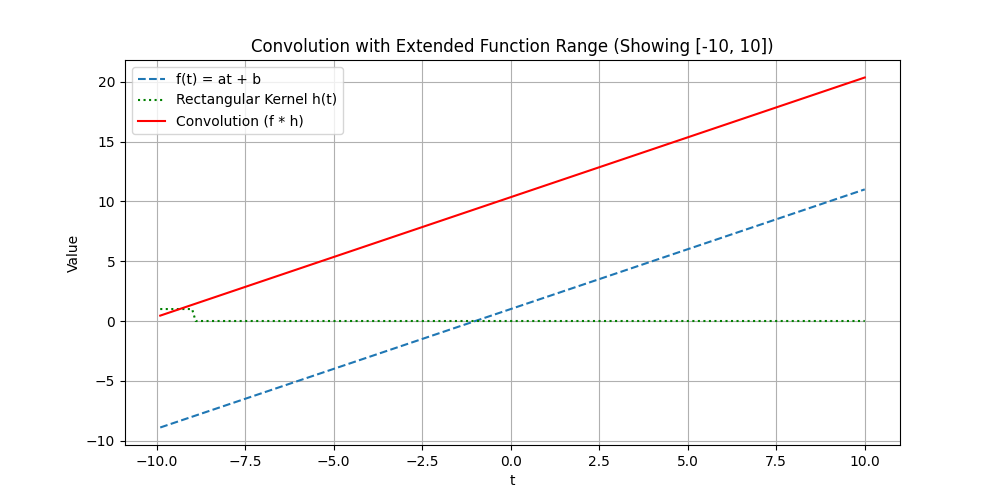
\includegraphics[width=0.6\textwidth]{figsm/5.png}
    \caption{$t_0 = 10$}
    \label{fig:conv_sinc}
\end{figure}
\begin{figure}[h]
    \centering
    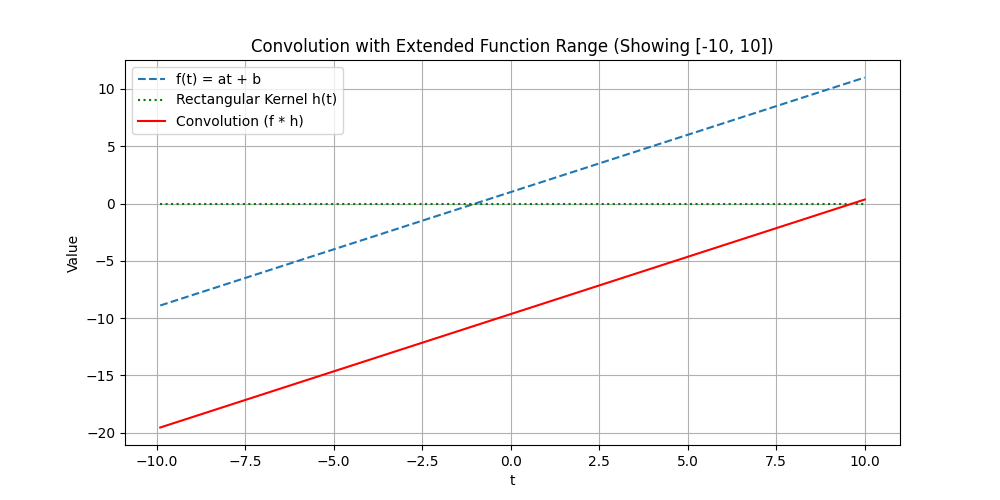
\includegraphics[width=0.6\textwidth]{figsm/6.png}
    \caption{$t_0 = -10$}
    \label{fig:conv_sinc}
\end{figure}
Shifting of the kernel by 10 units results in shifting of convoluted function by 10 units.

\section{Convolution of Exponential Functions}
	Let's choose $f(t) = e^{-at}$ for $a > 0$ as our input signal.
	
	The convolution is:
	\begin{equation}
		y(t) = \int_{-\infty}^{\infty} e^{-a\tau} \cdot h(t - \tau) d\tau
	\end{equation}
	
	Since $h(t - \tau)$ is non-zero only when $-T \leq t - \tau \leq T$, or $t - T \leq \tau \leq t + T$, the effective integration limits are:
	\begin{equation}
		y(t) = \int_{t-T}^{t+T} e^{-a\tau} d\tau
	\end{equation}
	
	Computing this integral:
	\begin{align}
		y(t) &= \int_{t-T}^{t+T} e^{-a\tau} d\tau \\
		&= \left[ -\frac{1}{a}e^{-a\tau} \right]_{t-T}^{t+T} \\
		&= \frac{e^{-at}}{a}(e^{aT} - e^{-aT})
	\end{align}
	
	Using the definition of hyperbolic sine, we can write:
	\begin{equation}
		y(t) = \frac{2\sinh(aT)}{a}e^{-at}
	\end{equation}
	
	\begin{figure}[htbp]
		\centering
		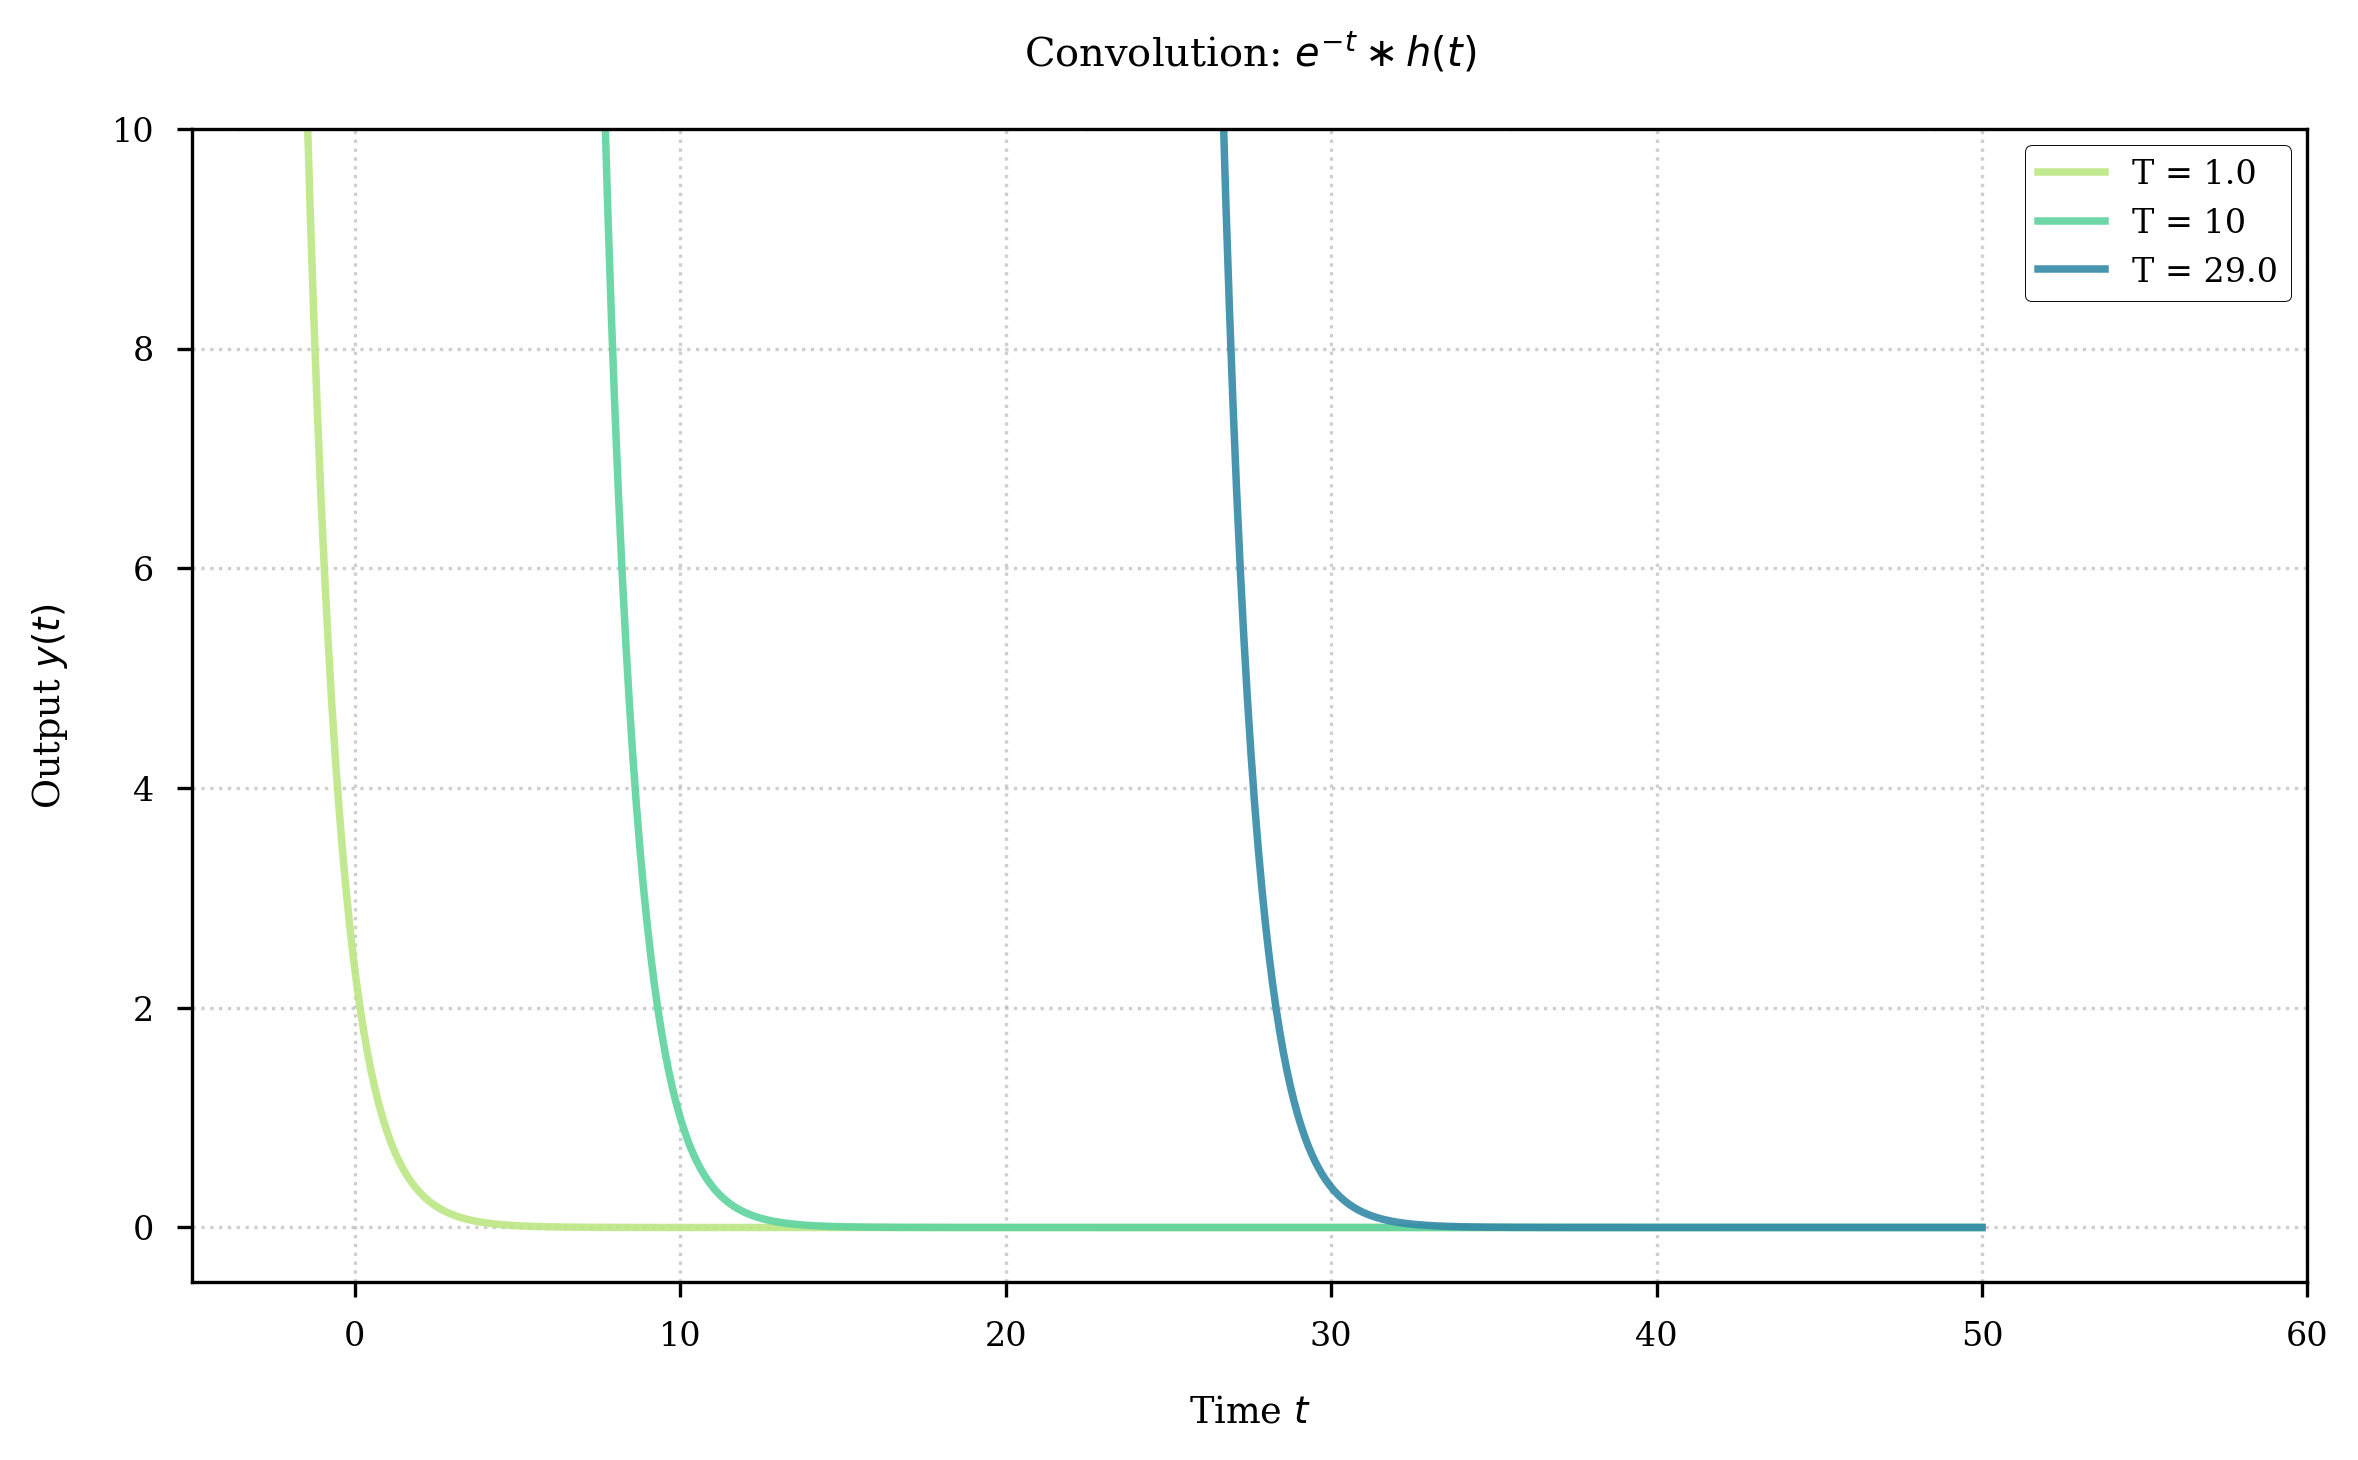
\includegraphics[width=0.8\textwidth]{figs/exp_convolution.png}
		\caption{Convolution of $f(t) = e^{-t}$ with a rectangular kernel for varying values of $T$. As $T$ increases, the output signal amplitude scales by $\frac{2\sinh(aT)}{a}$ but retains the exponential decay nature. For large values of $T$ (e.g., $T = 29.0$), the output achieves relatively higher amplitudes (approximately 8) than smaller $T$ values, showing the amplification property of the width of the rectangular kernel without losing the exponential nature of the original function.}
		\label{fig:exp_convolution}
	\end{figure}
	
	\section{Convolution with Hyperbolic Function}
	Let's consider $f(t) = \sinh(bt)$ for $b > 0$.
	
	The convolution is:
	\begin{equation}
		y(t) = \int_{-\infty}^{\infty} \sinh(b\tau) \cdot h(t - \tau) d\tau = \int_{t-T}^{t+T} \sinh(b\tau) d\tau
	\end{equation}
	
	Computing this integral:
	\begin{align}
		y(t) &= \int_{t-T}^{t+T} \sinh(b\tau) d\tau \\
		&= \left[ \frac{1}{b}\cosh(b\tau) \right]_{t-T}^{t+T} \\
		&= \frac{1}{b}(\cosh(b(t+T)) - \cosh(b(t-T)))
	\end{align}
	
	Using the identity $\cosh(A) - \cosh(B) = 2\sinh(\frac{A+B}{2})\sinh(\frac{A-B}{2})$:
	\begin{align}
		y(t) &= \frac{1}{b}(2\sinh(bt)\sinh(bT)) \\
		&= \frac{2\sinh(bT)}{b}\sinh(bt)
	\end{align}
	
	\begin{figure}[htbp]
		\centering
		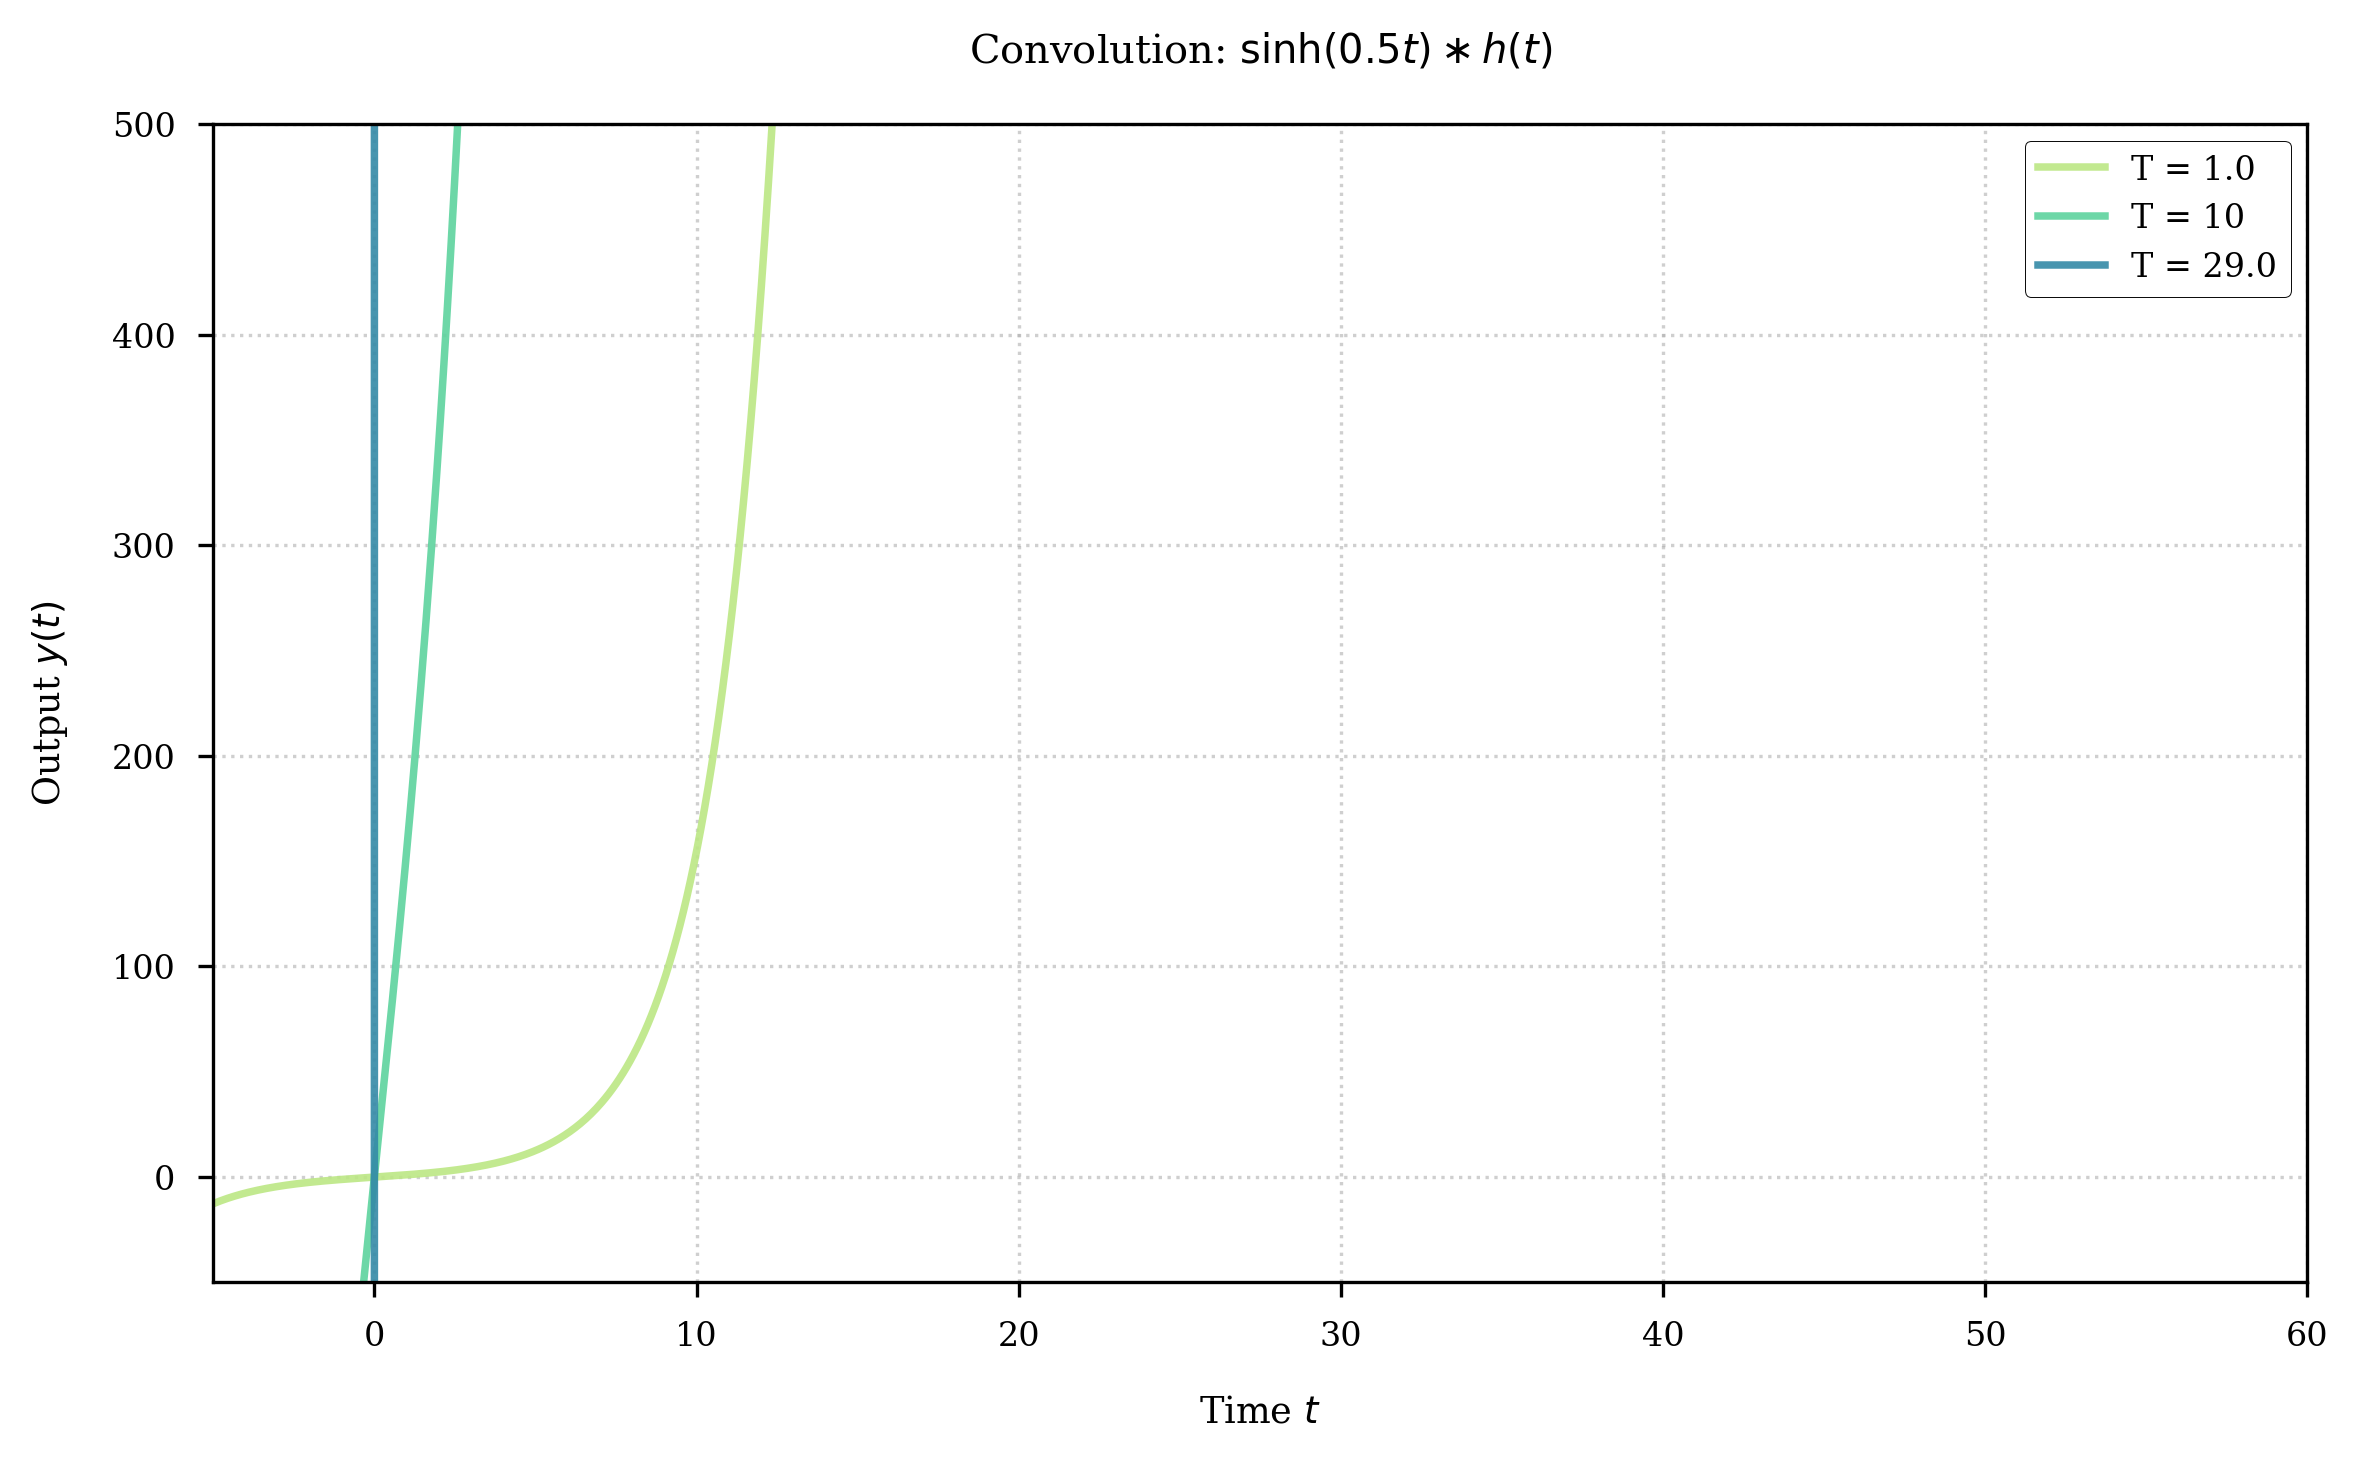
\includegraphics[width=0.8\textwidth]{figs/hyper_convolution.png}
		\caption{Convolution of $f(t) = \sinh(0.5t)$ with a rectangular kernel of varying $T$. The output retains the hyperbolic sine form but with increased magnitude that varies with $\frac{2\sinh(bT)}{b}$. With an increase in $T$, the amplitude increases significantly, reaching around $\pm100$ for $T = 29.0$. In contrast to the exponential scenario, this output increases both positively and negatively, illustrating the way the wider rectangular kernels increase the hyperbolic nature of the original function.}
		\label{fig:hyper_convolution}
	\end{figure}
	
	\subsection{Modified Kernel Analysis}
	\subsubsection{Kernel for $t > 0$ (Part a)}
	For part (a), we need to modify the kernel to only consider the part for $t > 0$:
	\begin{equation}
		h_m(t) = 
		\begin{cases} 
			1, & \text{for } 0 \leq t \leq T \\
			0, & \text{otherwise}
		\end{cases}
	\end{equation}
	
	This is equivalent to applying a unit step function to the original kernel and adjusting the range:
	\begin{equation}
		h_m(t) = h(t+T) \cdot u(t)
	\end{equation}
	
	For the exponential function $f(t) = e^{-at}$, we now need to introduce the step function $u(t)$ for a causal system analysis. Let's define $f_c(t) = e^{-at}u(t)$ for $a > 0$.
	
	The convolution becomes:
	\begin{equation}
		y_m(t) = \int_{-\infty}^{\infty} e^{-a\tau}u(\tau) \cdot h_m(t - \tau) d\tau
	\end{equation}
	
	The effective integration limits are determined by where both $\tau \geq 0$ and $0 \leq t - \tau \leq T$, or $t - T \leq \tau \leq t$ and $\tau \geq 0$:
	\begin{equation}
		y_m(t) = \int_{\max(0, t-T)}^{\min(t, t)} e^{-a\tau} d\tau
	\end{equation}
	
	Analyzing different cases:
	
	\subsubsection{Case 1: $t < 0$}
	In this case, $\min(t, t) = t < 0$, so there's no overlap and $y_m(t) = 0$.
	
	\subsubsection{Case 2: $0 \leq t < T$}
	Here, $t - T < 0$ and $t \geq 0$, so:
	\begin{align}
		y_m(t) &= \int_{0}^{t} e^{-a\tau} d\tau \\
		&= \frac{1}{a}(1 - e^{-at})
	\end{align}
	
	\subsubsection{Case 3: $t \geq T$}
	Both $t - T \geq 0$ and $t > 0$, so:
	\begin{align}
		y_m(t) &= \int_{t-T}^{t} e^{-a\tau} d\tau \\
		&= \frac{1}{a}(e^{-a(t-T)} - e^{-at}) \\
		&= \frac{e^{-at}}{a}(e^{aT} - 1)
	\end{align}
	
	Therefore, the complete convolution result for the modified kernel is:
	\begin{equation}
		y_m(t) = 
		\begin{cases} 
			0, & t < 0 \\
			\frac{1}{a}(1 - e^{-at}), & 0 \leq t < T \\
			\frac{e^{-at}}{a}(e^{aT} - 1), & t \geq T
		\end{cases}
	\end{equation}
	
	\begin{figure}[htbp]
		\centering
		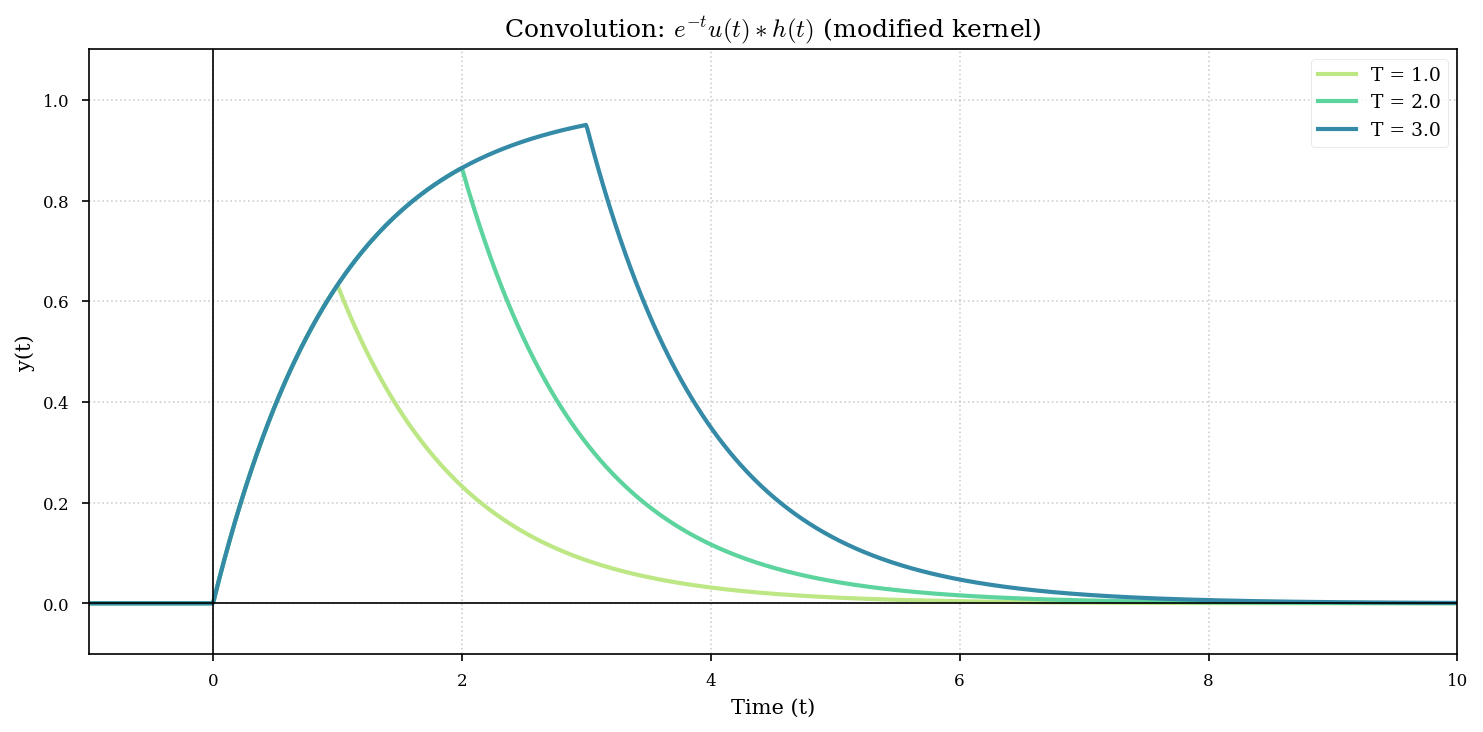
\includegraphics[width=0.8\textwidth]{figs/exp_modified_convolution.png}
		\caption{Convolution of $f(t) = e^{-t}u(t)$ with the modified kernel for various values of $T$. The result is zero for $t < 0$ due to causality. For $0 \leq t < T$, the response rises as $(1 - e^{-at})/a$ to various maximum levels depending on $T$. For $t \geq T$, the output takes an exponential decay form $e^{-at}(e^{aT} - 1)/a$. Higher values of $T$ produce greater peak amplitudes and broader response regions. For $T = 3.0$, the peak is about 0.95 at $t \approx 3$, with exponential decay thereafter.}
		\label{fig:exp_modified_convolution}
	\end{figure}
	
	\subsection{Hyperbolic Function with Modified Kernel}
	For the hyperbolic function with the modified kernel, a similar analysis gives:
	
	\subsubsection{Case 1: $t < 0$}
	The output is zero: $y_m(t) = 0$.
	
	\subsubsection{Case 2: $0 \leq t < T$}
	\begin{align}
		y_m(t) &= \int_{0}^{t} \sinh(b\tau) d\tau \\
		&= \frac{1}{b}(\cosh(bt) - 1)
	\end{align}
	
	\subsubsection{Case 3: $t \geq T$}
	\begin{align}
		y_m(t) &= \int_{t-T}^{t} \sinh(b\tau) d\tau \\
		&= \frac{1}{b}(\cosh(bt) - \cosh(b(t-T)))
	\end{align}
	
	Using the identity $\cosh(A) - \cosh(B) = 2\sinh(\frac{A+B}{2})\sinh(\frac{A-B}{2})$:
	\begin{align}
		y_m(t) &= \frac{1}{b}(2\sinh(b(t-\frac{T}{2}))\sinh(\frac{bT}{2})) \\
		&= \frac{2\sinh(\frac{bT}{2})}{b}\sinh(b(t-\frac{T}{2}))
	\end{align}
	
	Therefore, the complete convolution result is:
	\begin{equation}
		y_m(t) = 
		\begin{cases} 
			0, & t < 0 \\
			\frac{1}{b}(\cosh(bt) - 1), & 0 \leq t < T \\
			\frac{2\sinh(\frac{bT}{2})}{b}\sinh(b(t-\frac{T}{2})), & t \geq T
		\end{cases}
	\end{equation}
	
	\begin{figure}[htbp]
		\centering
		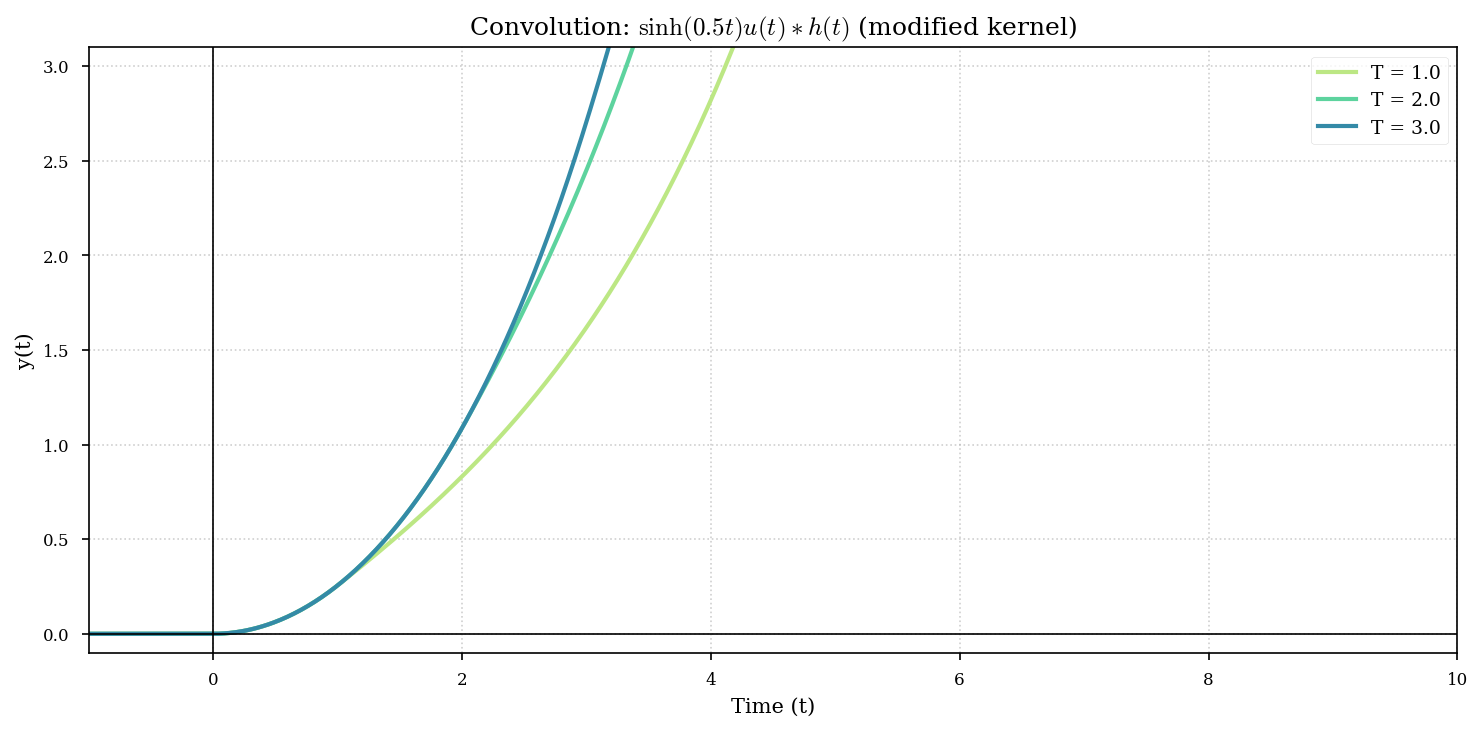
\includegraphics[width=0.8\textwidth]{figs/hyper_modified_convolution.png}
		\caption{Convolution of $f(t) = \sinh(0.5t)u(t)$ with the modified kernel for various values of $T$. The result is zero for $t < 0$, and for $t > 0$ has exponential growth properties of the hyperbolic sine function. As $T$ grows, the rate of growth becomes faster, with the $T = 3.0$ curve having the most rapid growth. In contrast to the exponential case, these curves still rise without limit after $t = T$, with the pattern $\frac{2\\sinh(\frac{bT}{2})}{b}\sinh(b(t-\frac{T}{2}))$. All three curves approach each other for small $t$ but spread out considerably as $t$ grows, illustrating how the system exaggerates the input signal more with wider kernels.}
		\label{fig:hyper_modified_convolution}
	\end{figure}
	
	\subsection{Time-Shifted Kernel (Part b)}
	For part (b), we analyze a kernel shifted by a time $\tau_0$:
	\begin{equation}
		h_s(t) = 
		\begin{cases} 
			1, & \text{for } -T+\tau_0 \leq t \leq T+\tau_0 \\
			0, & \text{otherwise}
		\end{cases}
	\end{equation}
	
	This is equivalent to:
	\begin{equation}
		h_s(t) = h(t-\tau_0)
	\end{equation}
	
	\subsubsection{Exponential Function with Time-Shifted Kernel}
	The convolution with $f(t) = e^{-at}$ becomes:
	\begin{equation}
		y_s(t) = \int_{-\infty}^{\infty} e^{-a\tau} \cdot h_s(t - \tau) d\tau = \int_{-\infty}^{\infty} e^{-a\tau} \cdot h(t - \tau - \tau_0) d\tau
	\end{equation}
	
	Using the time-shifting property of convolution, we can write:
	\begin{equation}
		y_s(t) = y(t-\tau_0) = \frac{2\sinh(aT)}{a}e^{-a(t-\tau_0)} = \frac{2\sinh(aT)}{a}e^{a\tau_0}e^{-at}
	\end{equation}
	
	This shows that shifting the kernel by $\tau_0$ results in a time-shift of the output and an amplitude scaling by $e^{a\tau_0}$.
	
	\begin{figure}[htbp]
		\centering
		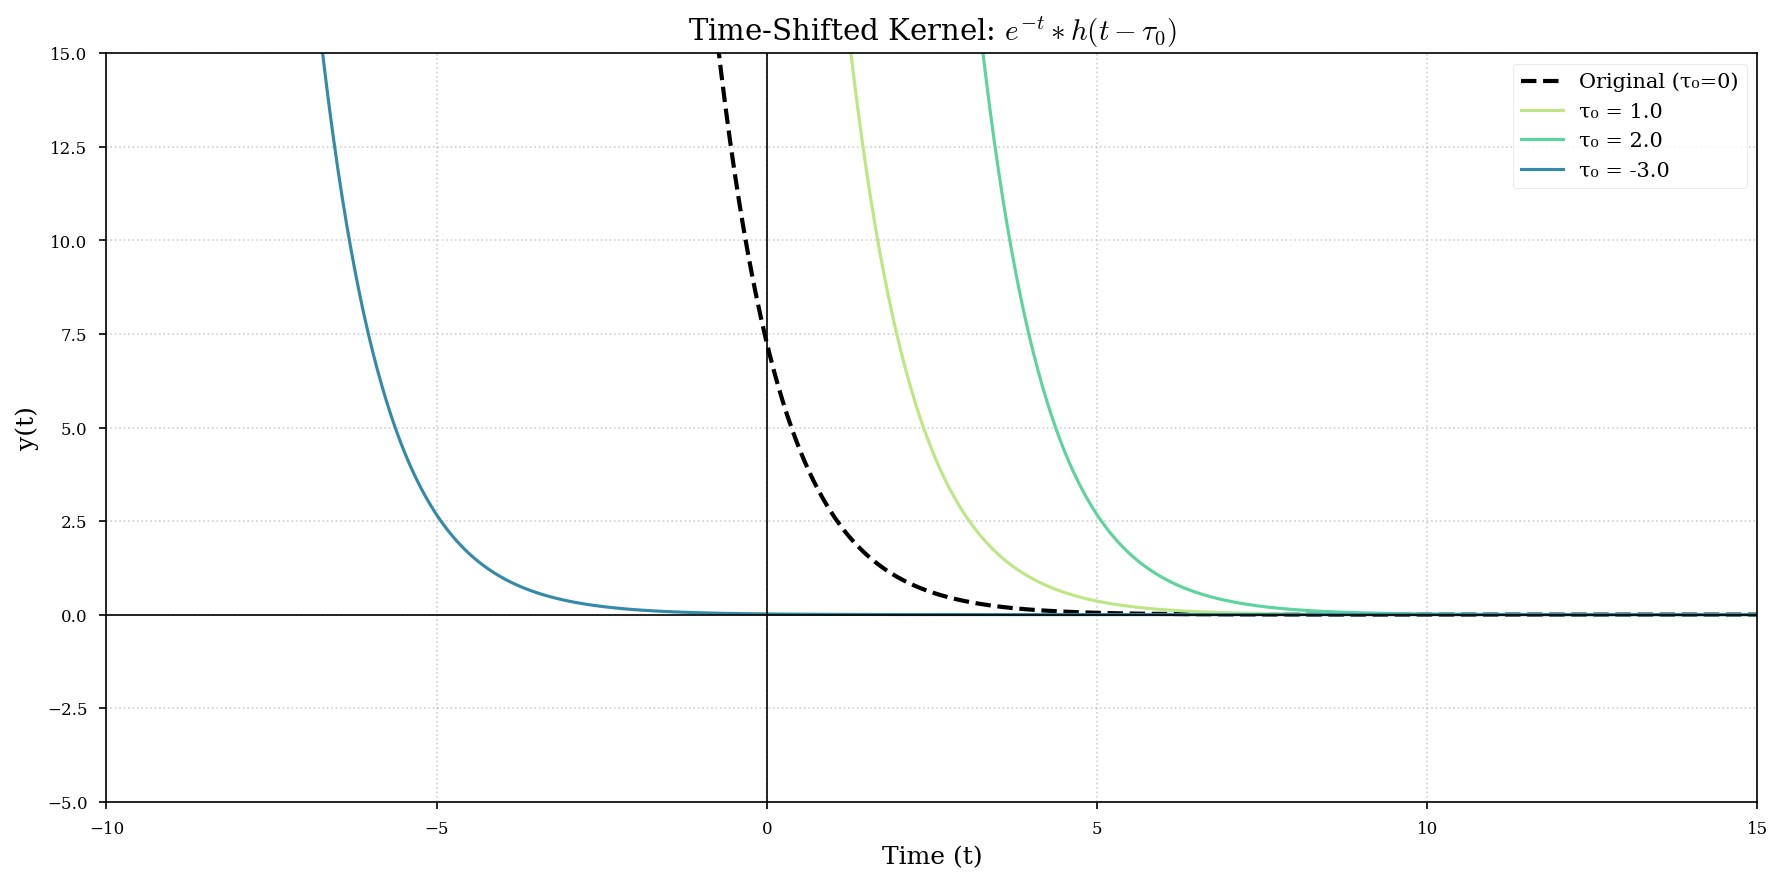
\includegraphics[width=0.8\textwidth]{figs/exp_time_shift_extended.png}
		\caption{Convolution of $f(t) = e^{-t}$ with time-shifted rectangular kernel $h(t-\tau_0)$ for various values of $\tau_0$. The original response ($\tau_0 = 0$) is represented as a dashed line. As $\tau_0$ is increased, the whole response curve is shifted to the right by $\tau_0$ and scaled by a factor of $e^{\tau_0}$. For $\tau_0 = 1.0$, the curve is shifted right by 1 unit and scales up in amplitude. For $\tau_0 = 2.0$, the shift is 2 units with additional amplification. Similarly, for $\tau_0 = -3.0$, the shift is 3 units to the left. All curves share the typical exponential decay but different initial points and amplitudes, according to the equation $\frac{2\sinh(aT)}{a}e^{a\tau_0}e^{-at}$.}
		\label{fig:exp_shifted_kernel}
	\end{figure}
	
	\subsubsection{Hyperbolic Function with Time-Shifted Kernel}
	For the hyperbolic function $f(t) = \sinh(bt)$, the convolution with the time-shifted kernel is:
	\begin{equation}
		y_s(t) = \int_{-\infty}^{\infty} \sinh(b\tau) \cdot h_s(t - \tau) d\tau = \int_{-\infty}^{\infty} \sinh(b\tau) \cdot h(t - \tau - \tau_0) d\tau
	\end{equation}
	
	Using the time-shifting property of convolution, the result is:
	\begin{equation}
		y_s(t) = y(t-\tau_0) = \frac{2\sinh(bT)}{b}\sinh(b(t-\tau_0))
	\end{equation}
	
	This represents a pure time-shift of the original response without amplitude scaling, unlike the exponential case.
	
	\begin{figure}[htbp]
		\centering
		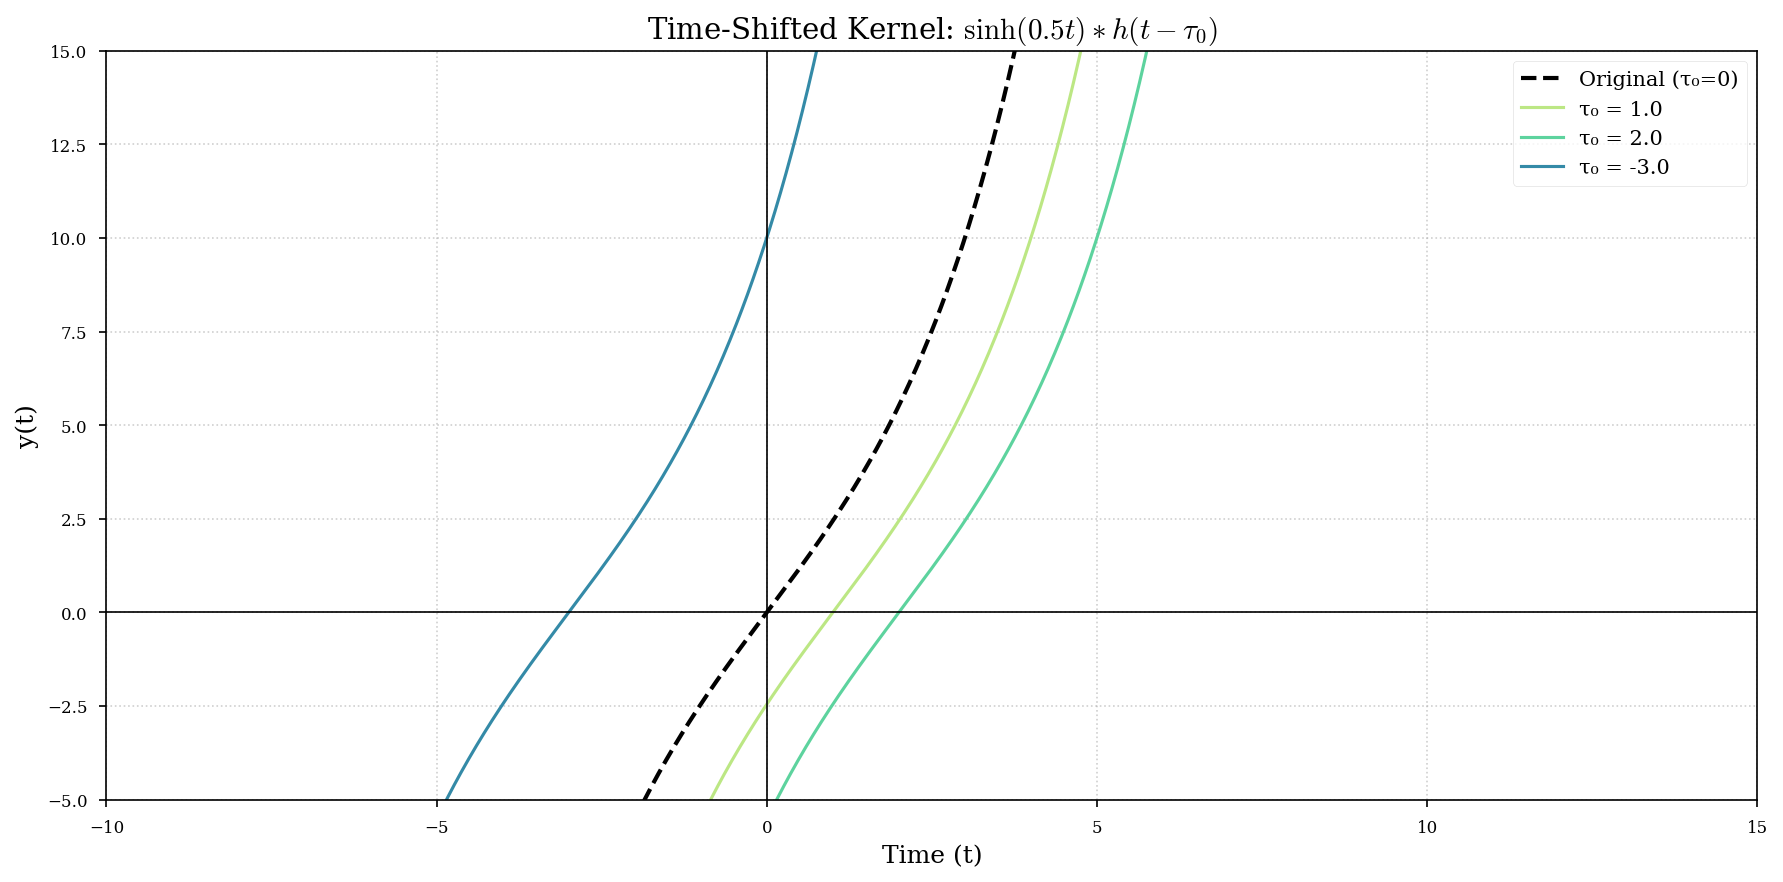
\includegraphics[width=0.8\textwidth]{figs/hyper_time_shift_extended.png}
		\caption{Convolution of $f(t) = \sinh(0.5t)$ with time-shifted rectangular kernel $h(t-\tau_0)$ for various values of $\tau_0$. The original response ($\tau_0 = 0$) is a dashed line. For increasing values of $\tau_0$, the response curves move horizontally to the right by $\tau_0$ units. For $\tau_0 = 1.0$, the curve moves right by 1 unit, for $\tau_0 = 2.0$, the move is 2 units and for $\tau_0 = -3.0$, its 3 units to the left. In contrast to the exponential case, there is no scaling of amplitude - just a simple time-shift, as seen in the parallel curves. Every curve is described by the equation $\frac{2\sinh(bT)}{b}\sinh(b(t-\tau_0))$, with the same hyperbolic growth rate but with varying x-intercepts at $t = \tau_0$.}
	\end{figure}
	
	\subsection{Comparison of Exponential and Hyperbolic Functions with Time-Shifted Kernels}
	The time-shifted kernel brings out the key distinction between exponential and hyperbolic functions in convolution systems:
	
	
	\begin{itemize}
		\item For the exponential function $f(t) = e^{-at}$, a time-shift in the kernel results in both a time-shift and amplitude scaling in the output. The scaling factor $e^{a\\tau_0}$ grows exponentially with the amount of the shift.
		\item For the hyperbolic function $f(t) = \sinh(bt)$, a time-shift in the kernel results only in a time-shift in the output and not in amplitude scaling. The curves do not change their shape and are merely shifted horizontally.
	\end{itemize}


\section{Convolution of sinc function}

Given kernel, 
\begin{align}
h(t) =
\begin{cases}
1, & \text{for } -T \leq t \leq T \\
0, & \text{otherwise}
\end{cases} \label{eq:kernel}
\end{align}
and the function 
\begin{align*}
f(t) &= sinc(t) \\
     &= \frac{sint}{t}
\end{align*}
Let $y(t) = x(t) * f(t)$, then
\begin{align*}
	y(t) &= h(t) * f(t) \\
             &= f(t) * h(t) \\
             &= \int_{-\infty}^{\infty} f(\tau) h(t - \tau) d \tau \\
\end{align*}
\[
h(t - \tau) =
\begin{cases}
1, & \text{for } -T \leq t - \tau \leq T \\
0, & \text{otherwise}
\end{cases}
\]
\[
h(t - \tau) =
\begin{cases}
1, & \text{for } \tau - T \leq t \leq \tau + T \\
0, & \text{otherwise}
\end{cases}
\]
Therefore, the convolution becomes, 
\begin{align*}
	y(t) &= \int_{t - T}^{t + T} \frac{sin(\tau)}{\tau} * 1 d\tau \\
	y(t) &= \int_{t - T}^{t + T} \frac{sin(\tau)}{\tau} d\tau
\end{align*}
This integration can be numerically computed and can be seen to be the following - \\
\begin{figure}[!ht]
    \centering
    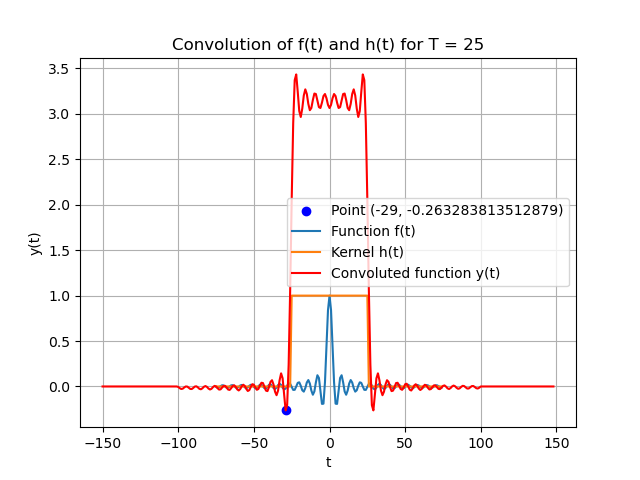
\includegraphics[width=0.6\textwidth]{figs/Conv_sinc.png}
    \caption{T = 25}
    \label{fig:conv_sinc}
\end{figure}
\newpage
For different values of T, the change in $y(t)$ is depicted in the following - \\
\begin{figure}[h]
    \centering
    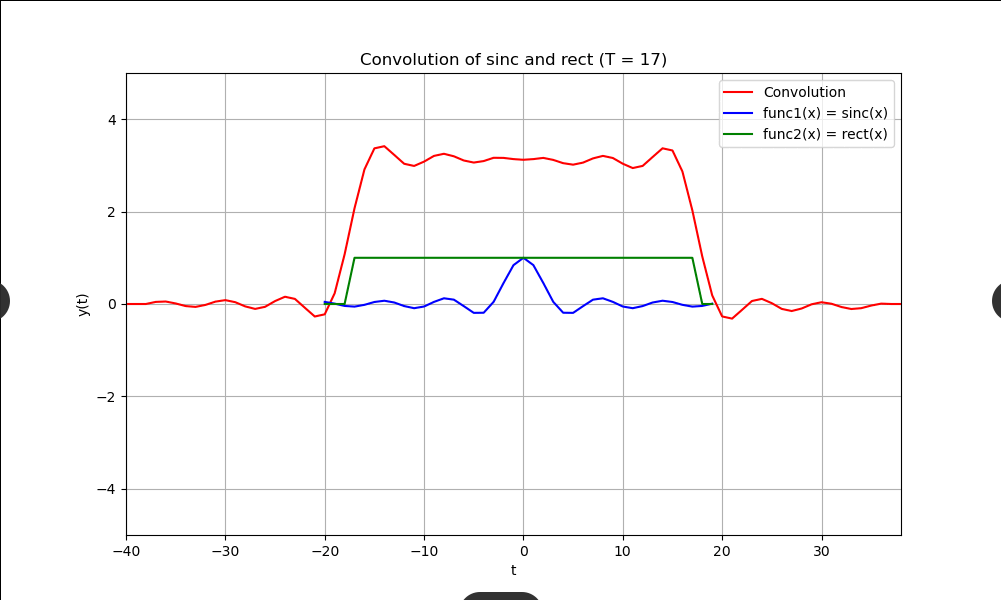
\includegraphics[width=0.6\textwidth]{figs/con1.png}
    \caption{T = 17}
    \label{fig:conv_sinc}
\end{figure}
\begin{figure}[h]
    \centering
    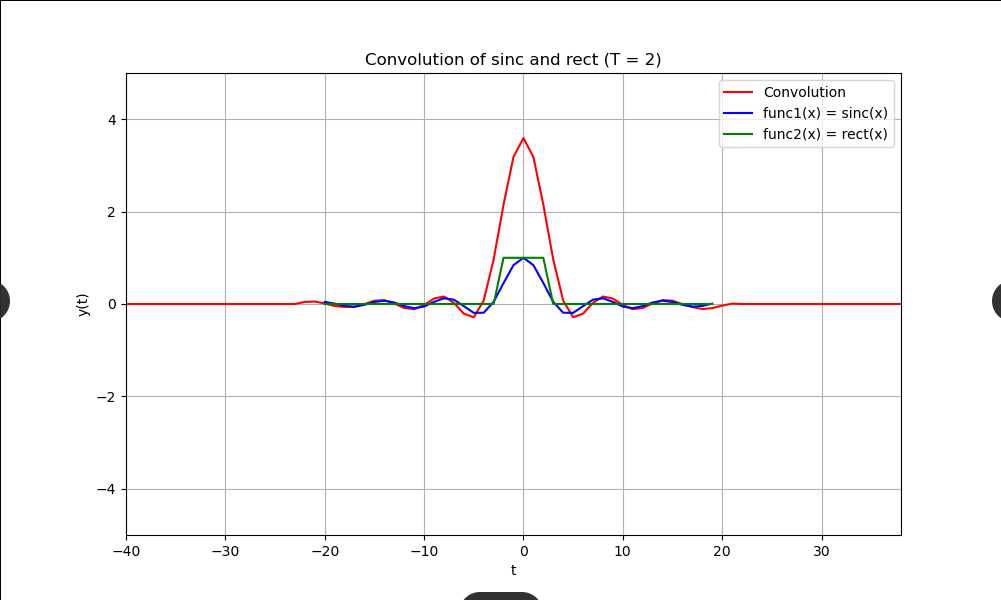
\includegraphics[width=0.6\textwidth]{figs/con2.png}
    \caption{T = 2}
    \label{fig:conv_sinc}
\end{figure}
\begin{figure}[h]
    \centering
    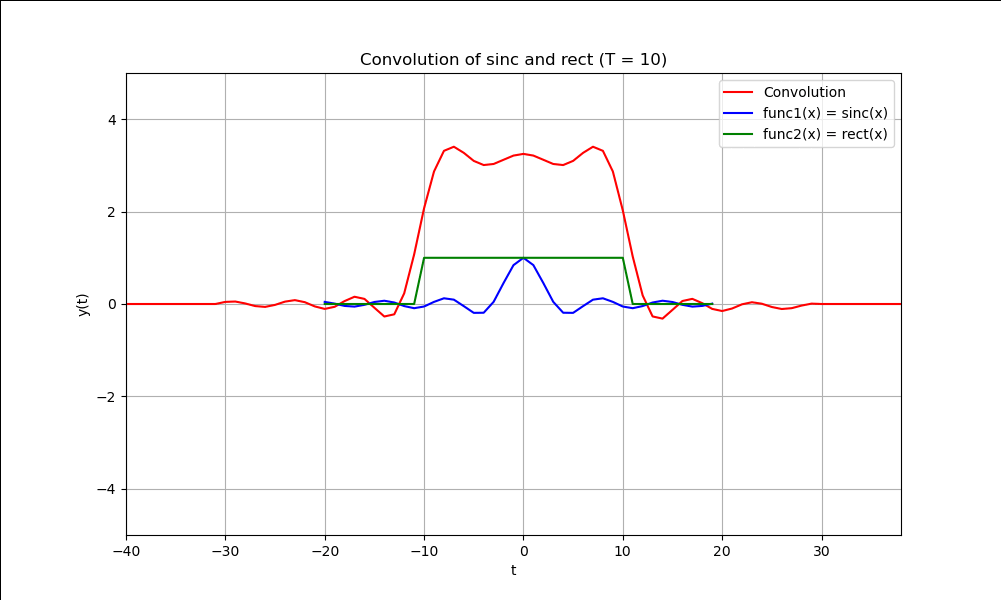
\includegraphics[width=0.6\textwidth]{figs/con3.png}
    \caption{T = 10}
    \label{fig:conv_sinc}
\end{figure}
\begin{figure}[h]
    \centering
    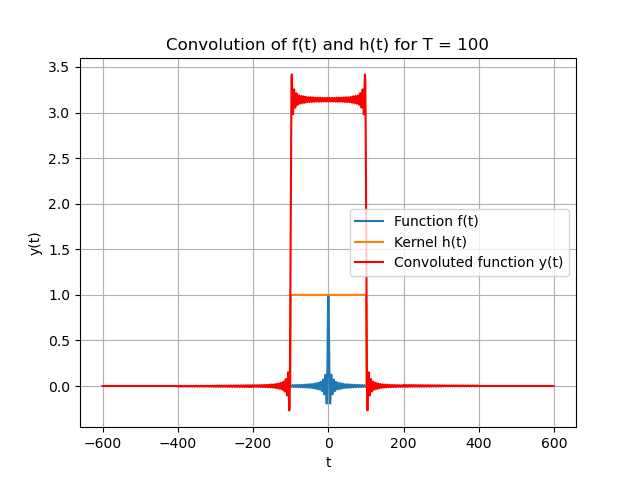
\includegraphics[width=0.6\textwidth]{figs/con4.png}
    \caption{T = 100}
    \label{fig:conv_sinc}
\end{figure}
\begin{figure}[h]
    \centering
    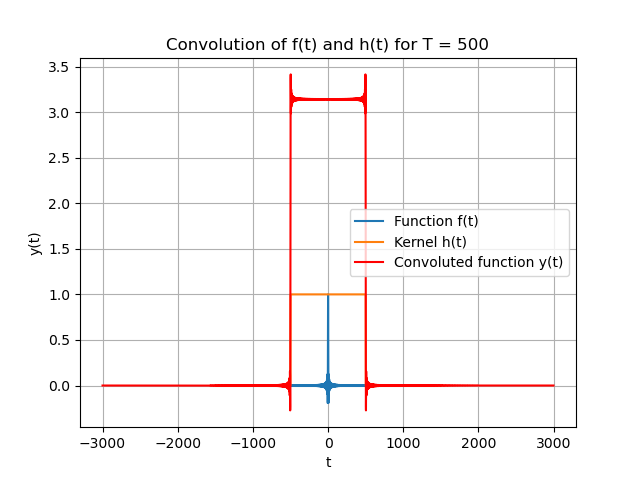
\includegraphics[width=0.6\textwidth]{figs/con5.png}
    \caption{T = 500}
    \label{fig:conv_sinc}
\end{figure}
\newpage
It can be seen that as $T$ increases, $y(t)$ becomes more square.

\newpage
\subsection{Considering the kernel for $t>0$}
The response of the system for different values of $T$ are as follows - \\
\begin{figure}[h]
    \centering
    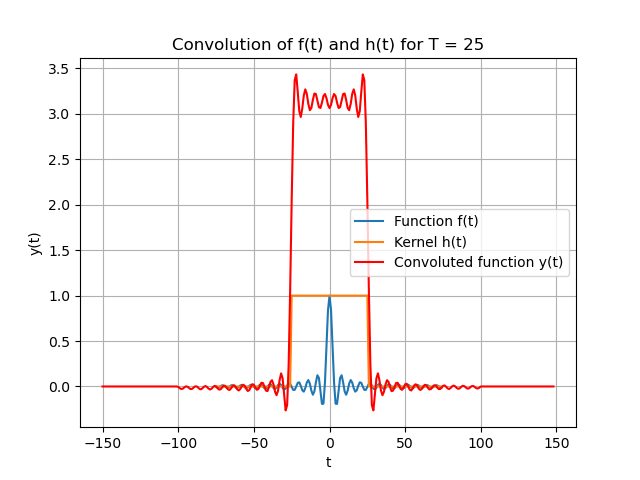
\includegraphics[width=0.6\textwidth]{figs/conv_sinc.png}
    \caption{T = 25}
    \label{fig:conv_sinc}
\end{figure}
\begin{figure}[h]
    \centering
    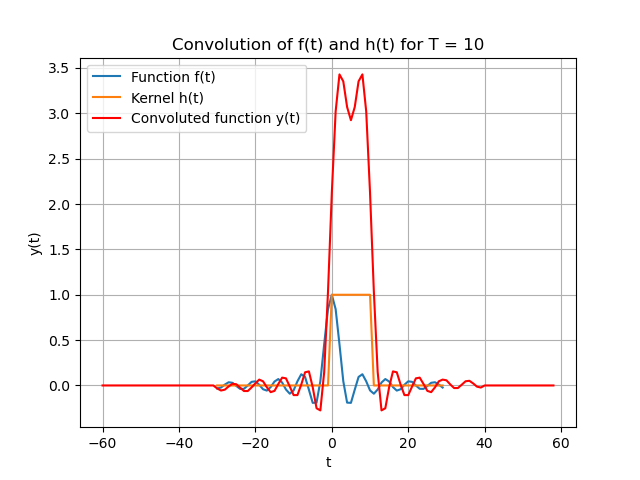
\includegraphics[width=0.6\textwidth]{figs/con6.png}
    \caption{T = 10}
    \label{fig:conv_sinc}
\end{figure}
\begin{figure}[h]
    \centering
    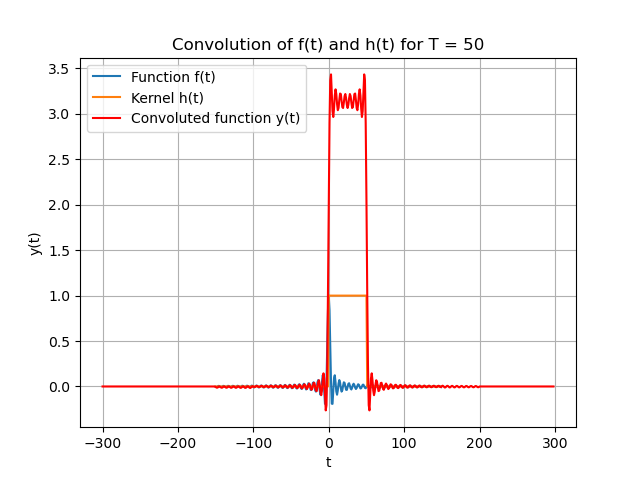
\includegraphics[width=0.6\textwidth]{figs/con7.png}
    \caption{T = 50}
    \label{fig:conv_sinc}
\end{figure}
\begin{figure}[h]
    \centering
    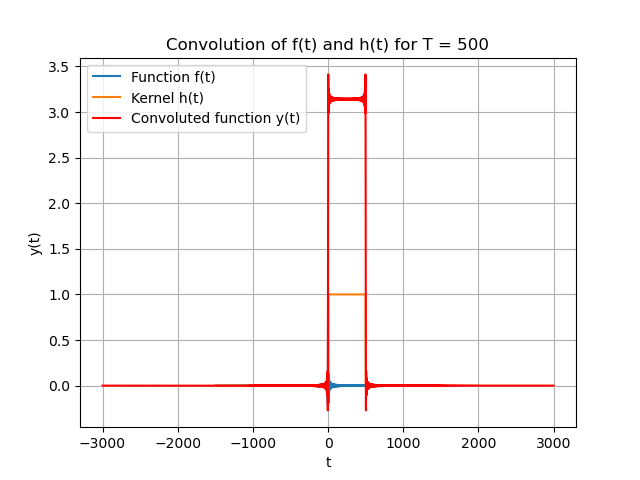
\includegraphics[width=0.6\textwidth]{figs/con8.png}
    \caption{T = 500}
    \label{fig:conv_sinc}
\end{figure}
It can be seen that the width of the convolution becomes half and it becomes shifted to the right.
\newpage

\subsection{Shifting the kernel by $t_{0}$}
Shifting of kernel means moving the kernel to the left or right by an amount, i.e., if the given kernel is shifted by an amount $t_0$, then it becomes, 
\[
h(t) =
\begin{cases}
1, & \text{for } -T \leq t-t_0 \leq T \\
0, & \text{otherwise}
\end{cases}
\]
\[
h(t) =
\begin{cases}
1, & \text{for } -T+t_0 \leq t \leq T+t_0 \\
0, & \text{otherwise}
\end{cases}
\]
If we are convolving a signal with the kernel, at each time $t$, we are sliding the kernel over the signal and computing how much they overlap. So, when we shift the kernel by $t_0$, we are changing when the kernel has its maximum influence.
This can physically mean applying a response $t_0$ time units early (or) $t_0$ time units late depending upon the sign of $t_0$, i.e., if $t_0 > 0$, the response is delayed and is advanced for $t_0 < 0$. This results in the convoluted signal also to be shifted by the same amount, as in figures \ref{fig:rshift} and \ref{fig:lshift} - 
\begin{figure*}[!htb]
    {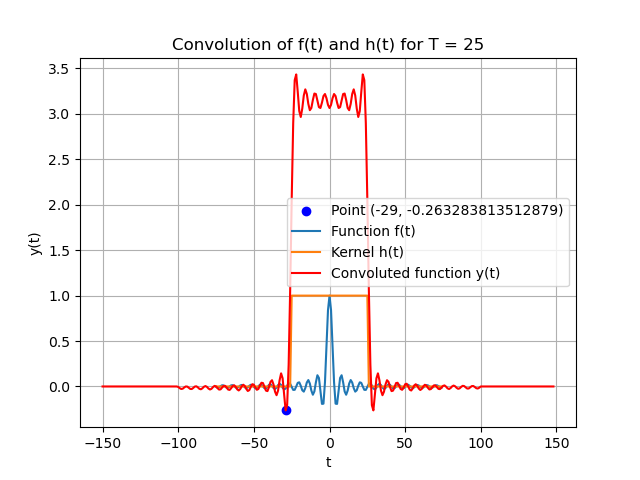
\includegraphics[ width=0.40\textwidth]{figs/Conv_sinc.png}}
    \hspace{\fill}
    {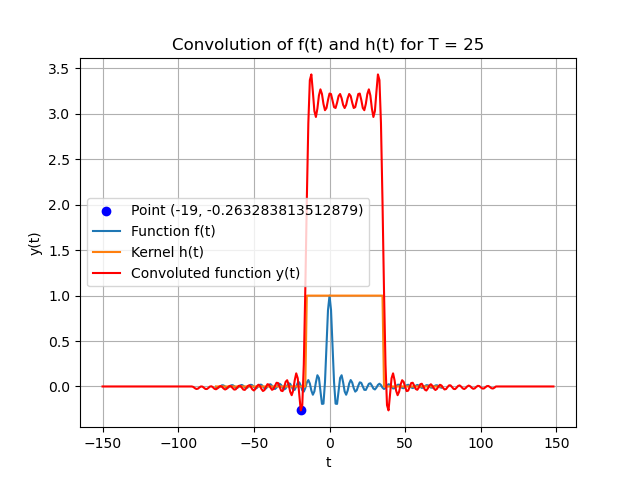
\includegraphics[ width=0.40\textwidth]{figs/conv_shift.png}}
    \hspace{\fill}\\
    \caption{Shifting toward right}
    \label{fig:rshift}
\end{figure*}
\begin{figure*}[!htb]
    {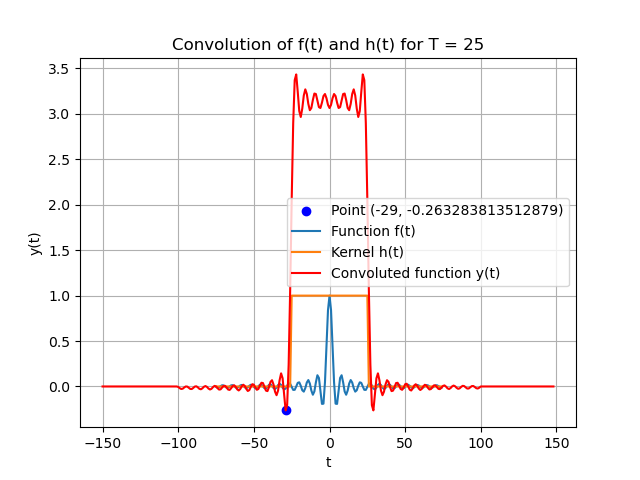
\includegraphics[ width=0.40\textwidth]{figs/Conv_sinc.png}}
    \hspace{\fill}
    {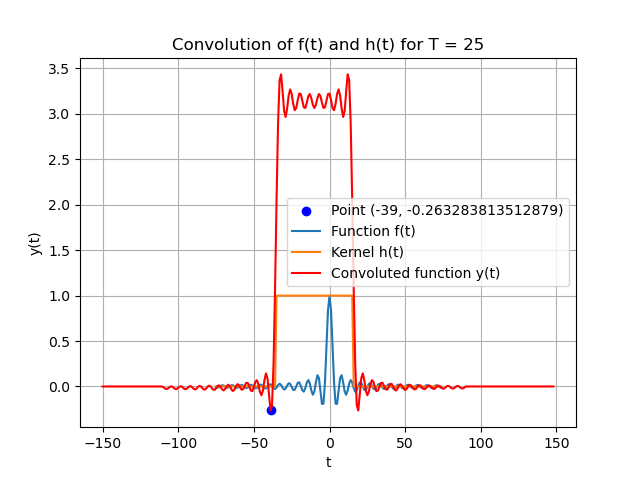
\includegraphics[ width=0.40\textwidth]{figs/conv_left.png}}
    \hspace{\fill}\\
    \caption{Shifting toward left}
    \label{fig:lshift}
\end{figure*}
Shifting of the kernel by 10 units results in shifting of convoluted function by 10 units.
\newpage






	     

\documentclass[12pt]{article}
\usepackage{graphicx}
\usepackage{geometry}
\usepackage{fancyhdr}
\usepackage{titling} 
\usepackage{amsmath}  
\usepackage{amssymb}  
\usepackage{enumitem} 
\usepackage{xcolor}   
\usepackage{circuitikz}
\usepackage{animate}
\usepackage{algorithm}
\usepackage{algpseudocode}
% Set margins
\geometry{a4paper, margin=1in}

% Title, name, and date
\title{\textbf{EE1060 - DETT GROUP QUIZ 2}}
\author{EE24BTECH11012 - Bhavanisankar G S}
\date{\today}

% Add logo to the title
\begin{document}

% First page with title, name, date, and logo
\maketitle
\thispagestyle{empty} % Remove page number from the first page

\newpage
\tableofcontents
\newpage

\section{\textbf{What is convolution ?}}

Convolution is a mathematical operation on two functions, $f$ and $g$, as the integral of the product of the two functions after one is reflected about the y-axis and shifted, i.e., If we are convolving a signal with a kernel, at each time $t$, we are sliding the kernel over the signal and computing how much they overlap. This is useful in various fields of study like finding the system response given the impulse response, signal processing and in probability.\\
Given two functions $f(x)$ and $g(x)$, convolution of the two signals, \\
\begin{align}
	x(t) &= f(t) * g(t) \\
	     &= \int_{-\infty}^{\infty} f(\tau) g(t - \tau) d \tau \label{eq:conv}
\end{align}
Some properties of convolution : \\
\begin{enumerate}
\item \textbf{Commutativity} : 
\begin{align*}
f(t) * g(t) &= g(t) * f(t)
\end{align*}
\item \textbf{Distributivity} :
\begin{align*}
f(t) * [g(t) + h(t)] &= [f(t) * g(t)] + [f(t) * h(t)] 
\end{align*}
\item \textbf{Associativity} :
\begin{align*}
f(t) * [g(t) * h(t)] &= [f(t) * g(t)] * h(t)
\end{align*}
\item \textbf{Time shifting property} :
If we are given $y(t) = x_1 (t) * x_2 (t)$, then
\begin{align*}
	x_1(t) * x_2(t - T) &= y(t - T) \\
ex_1(t - T) * x_2(t) &= y(t - T) \\
	x_1(t - T_1) * x_2(t - T_2) &= y(t - T_1 - T_2)
\end{align*}
\item \textbf{Width property} :
If the duration of signals $f(t)$ and $g(t)$ are $T_1$ and $T_2$ respectively, then the duration of signal convolving $f(t)$ and $g(t)$ is equal to $T_1 + T_2$
\end{enumerate}

\section{Discrete convolution}

Usually when dealing with real life signals, we don't have the complete function in but rather, discreet samples of the function. So it is also useful to look at the discrete convolution, which is given by,

\begin{align*}
    y[k] = (f*h)[k] = \sum_{m=0}^{\infty} f[m]h[m-k]
\end{align*}

Discrete colvolution follow all properties continuous convolution follows. we use this to numeically compute convolution of two signals.

\section{Convolution Theorem}

The convolution theorem states that,

If,
\begin{align*}
    (u*v)(t) = r(t)
\end{align*}

Then,
\begin{align*}
    \mathcal{L}\{r(t)\} = \mathcal{L}\{u(t)\}\mathcal{L}\{v(t)\}
\end{align*}

This provides a much faster way to compute convolution of the signals.

\section{Fast Fourier Transform (FFT) and it's inverse (IFFT)}

FFT is the algorithm used to find the fourier transform of a given signal. It is a recursive algorithm with a time complexity of $\mathcal{O}(n\log(n))$. To explain the algorithm and explain how convolution theorem works, we can explain it using product of two polynomials.

Let $P_1(x)$ and $P_2(x)$ be polynomials of degree $n$. Let $\vec{p_1}$ and $\vec{p_2}$ be the vectors, whose elements are the coefficients of $P_1(x)$ and $P_2(x)$.
If $P(x) = P_1(x)\times P_2(x)$, then the coefficients of $P(x)$ is the discrete convolution of $\vec{p_1}$ and $\vec{p_2}$. We can verify that with some algebra.

It is also known that, through $n$ unique points, there is a unique polynomial of degree $n$ passing through it. Using this property, let us choose $2n$ points on each of $P_1$ and $P_2$, with the x-coordinates. That will give us, $P_{1_p} = [(x_0, P_1(x_0)), (x_1, P_1(x_1), \dots)]$ and $P_{2_p} = [(x_0, P_2(x_0)), (x_1, P_2(x_1), \dots)]$, which we will call the point form of the polynomials. Now if we multiply the results, we will end up with $2n$ unique points that lie on $P(x)$ (i.e., $P_p = [(x_0, P_1(x_0)\times P_2(x_0)), (x_1, P_1(x_1)\times P_2(x_1)), \dots]$). Now if we find the polynomial that is passing through these points, that will give us the polynomial we needed all along.
In a nutshell, the process of finding the unique points on each polynomial to be multiplied is FFT and finding the equation of the polynomial from it's point form is IFFT.

Now, to find the point form by chosing random values of x and computing for each of them is pretty inefficient. Thus, we will look at something symmetric, so that the computations can be reduced.

Let,
\begin{align*}
    P(x) = a_0x^n + a_1x^{n-1} + \dots + a_n\\
    P(x) = P_e(x^2) + xP_o(x^2)\\
    P(-x) = P_e(x^2) -xP_o(x^2)
\end{align*}
where, $P_e(x)$ is the polynomial made only with the even terms of the original polynomial, and $P_o(x)$ is the polynomial made only with the odd terms of the polynomial, with the common $x$ term taken out.
With this, finding $P(x)$ for n points become simpler, as it will be enough to calulate $P_e$ and $P_o$ n/2 points. It would be really convenient if we could do such splitting for $P_e$ and $P_o$, but $x^2$ breaks the symmetry, and requires it to be complex. Well, whatif, we make it complex? And this is how the FFT algorithm works.

In the simplest case, where $n=2^k,k\in \mathbb{N}$, we take the $n/2^{th}$ root of 1, and recursively find $P_e$ and $P_o$.

The peudocode of FFT looks like the following:

\begin{algorithm}[!ht]
\caption{Fast Fourier Transform (FFT)}
\begin{algorithmic}[1]
\Procedure{FFT}{$x$}
    \State $n \gets |x|$ \Comment{Length of the input array}
    \If{$n = 1$} 
        \State \Return $x$
    \EndIf
    
    \State $\omega \gets e^{-2\pi i / n}$ \Comment{Note: negative exponent in Python code}
    \State $P_e \gets (x_0, x_2, \ldots, x_{n-2})$ \Comment{Even-indexed elements}
    \State $P_o \gets (x_1, x_3, \ldots, x_{n-1})$ \Comment{Odd-indexed elements}
    
    \State $y_e \gets \text{FFT}(P_e)$ \Comment{Recursive call on even-indexed elements}
    \State $y_o \gets \text{FFT}(P_o)$ \Comment{Recursive call on odd-indexed elements}
    
    \State $y \gets $ complex array of zeros of length $n$ \Comment{Initialize output array}
    \For{$i = 0$ to $n/2 - 1$}
        \State $y_i \gets y_e[i] + \omega^i \cdot y_o[i]$ \Comment{First half}
        \State $y_{i+n/2} \gets y_e[i] - \omega^i \cdot y_o[i]$ \Comment{Second half}
    \EndFor
    
    \State \Return $y$
\EndProcedure
\end{algorithmic}
\end{algorithm}

Now, that we finally know how to perform FFT, we can multiply the outputs to get the convolution. But there is a problem with the above algorithm. To calculate the convolution of 2 functions with n discrete samples, our convolved output will have 2n points. But the above algorithm gives n points, and thus multiplying the n points element wise, will only give us n points in the convolved signal. So, we need to modify it such that it gives us 2n points.


\begin{algorithm}[!ht]
\caption{Fast Fourier Transform (FFT) - For convolution}
\begin{algorithmic}[1]
\Procedure{FFT}{$x$}
    \State $n \gets |x|$ \Comment{Length of the input array}
    \If{$n = 1$} 
    \State \Return $(x, -x)$
    \EndIf
    
    \State $\omega \gets e^{-\pi i / n}$ \Comment{Note: observe it's $2n^{th}$ root of unity.}
    \State $P_e \gets (x_0, x_2, \ldots, x_{n-2})$ \Comment{Even-indexed elements}
    \State $P_o \gets (x_1, x_3, \ldots, x_{n-1})$ \Comment{Odd-indexed elements}
    
    \State $y_e \gets \text{FFT}(P_e)$ \Comment{Recursive call on even-indexed elements}
    \State $y_o \gets \text{FFT}(P_o)$ \Comment{Recursive call on odd-indexed elements}
    
    \State $y \gets $ complex array of zeros of length $n$ \Comment{Initialize output array}
    \For{$i = 0$ to $n - 1$}
        \State $y_i \gets y_e[i] + \omega^i \cdot y_o[i]$ \Comment{First half}
        \State $y_{i+n} \gets y_e[i] - \omega^i \cdot y_o[i]$ \Comment{Second half}
    \EndFor
    
    \State \Return $y$
\EndProcedure
\end{algorithmic}
\end{algorithm}


Now that we have the fourier transform of our signals, and multiplied them, we have the transformed version of the convolved signal. Now we have to apply the inverse Fourier Transform over it. How are we to do it?

Fourier Transform of a discreet signal can be considered as a matrix multiplication.


\begin{align*}
\begin{bmatrix}
    X(\omega^0)\\
    X(\omega^1)\\
    \vdots\\
    X(\omega^n)
\end{bmatrix} 
    &=
\begin{bmatrix}
    1      & 1      & \dots  & 1\\
    1      & \omega & \dots  & \omega^{n-1}\\
    \vdots & \vdots & \vdots & \vdots\\
    1      & \omega^{n-1} & \dots & \omega^{(n-1)(n-1)}
\end{bmatrix}
\begin{bmatrix}
    x_0\\
    x_1\\
    \vdots\\
    x_{n-1}
\end{bmatrix}\\
\begin{bmatrix}
    x_0\\
    x_1\\
    \vdots\\
    x_{n-1}
\end{bmatrix}
    &=
\begin{bmatrix}
    1      & 1      & \dots  & 1\\
    1      & \omega & \dots  & \omega^{n-1}\\
    \vdots & \vdots & \vdots & \vdots\\
    1      & \omega^{n-1} & \dots & \omega^{(n-1)(n-1)}
\end{bmatrix}^{-1}
\begin{bmatrix}
    X(\omega^0)\\
    X(\omega^1)\\
    \vdots\\
    X(\omega^n)
\end{bmatrix}\\
\begin{bmatrix}
    x_0\\
    x_1\\
    \vdots\\
    x_{n-1}
\end{bmatrix}
    &=
    \frac{1}{n}
\begin{bmatrix}
    1      & 1      & \dots  & 1\\
    1      & \omega^{-1} & \dots  & \omega^{-(n-1)}\\
    \vdots & \vdots & \vdots & \vdots\\
    1      & \omega^{-(n-1)} & \dots & \omega^{-(n-1)(n-1)}
\end{bmatrix}
\begin{bmatrix}
    X(\omega^0)\\
    X(\omega^1)\\
    \vdots\\
    X(\omega^n)
\end{bmatrix}\\
\end{align*}

Notice how the matrix looks very identical except that the roots of unity are inverted, and the whole matrix is divided by n. So with minor modifications to the FFT algorithm, we can perform IFFT too.

\begin{algorithm}
\caption{Inverse Fast Fourier Transform}
\begin{algorithmic}[1]
\Procedure{IFFT-Recursive}{$x$}
    \State $n \gets |x|$ \Comment{Length of the input array}
    \If{$n = 1$} 
        \State \Return $x$
    \EndIf
    
    \State $\omega \gets e^{2\pi i / n}$ \Comment{Note: opposite sign that of FFT for IFFT}
    \State $P_e \gets (x_0, x_2, \ldots, x_{n-2})$ \Comment{Even-indexed elements}
    \State $P_o \gets (x_1, x_3, \ldots, x_{n-1})$ \Comment{Odd-indexed elements}
    
    \State $y_e \gets \text{IFFT-Recursive}(P_e)$ \Comment{Recursive call on even-indexed elements}
    \State $y_o \gets \text{IFFT-Recursive}(P_o)$ \Comment{Recursive call on odd-indexed elements}
    
    \State $y \gets $ complex array of zeros of length $n$ \Comment{Initialize output array}
    \For{$i = 0$ to $n/2 - 1$}
        \State $y_i \gets y_e[i] + \omega^i \cdot y_o[i]$ \Comment{First half}
        \State $y_{i+n/2} \gets y_e[i] - \omega^i \cdot y_o[i]$ \Comment{Second half}
    \EndFor
    
    \State \Return $y$
\EndProcedure

\Procedure{IFFT}{$X$}
    \State $y \gets \text{IFFT-Recursive}(X)$
    \State \Return $y / |X|$ \Comment{Scale by $1/n$}
\EndProcedure
\end{algorithmic}
\end{algorithm}

\begin{figure}[H]
    \centering
    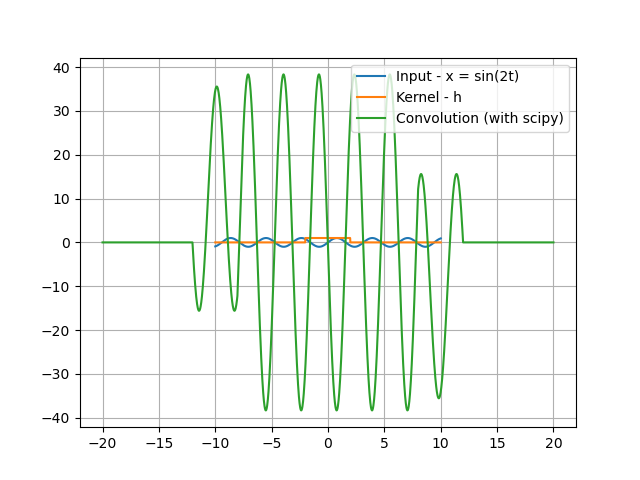
\includegraphics[width=0.7\linewidth]{figs/sci.png}
    \caption{Convolution by scipy}
\end{figure}

\begin{figure}[H]
    \centering
    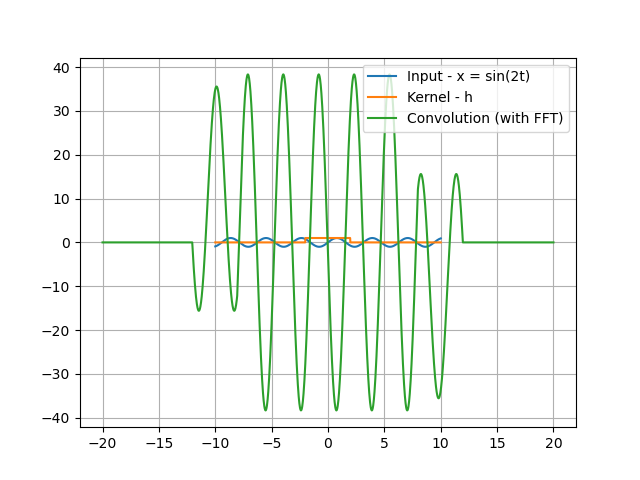
\includegraphics[width=0.7\linewidth]{figs/FFT.png}
    \caption{Convolution with python-implementation of FFT}
\end{figure}

\begin{figure}[H]
    \centering
    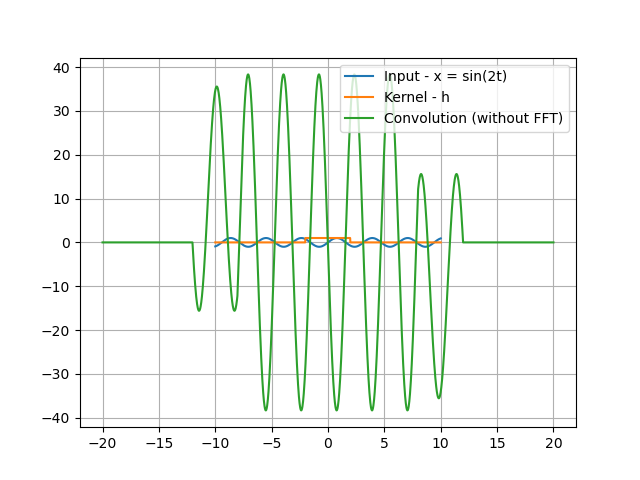
\includegraphics[width=0.7\linewidth]{figs/base.png}
    \caption{Convolution without FFT and IFFT algorithm}
\end{figure}

As we can see, the convolution matches. 


Now comparing the runtime of each algorithm,
\texttt{
Discreet Convolution:  0.33714938163757324\\
Scipy's Discreet Convolution 0.0010726451873779297\\
Discreen Convolution (FFT):  0.03110957145690918\\
}

Scipy's implementation is the fastest, as it is a professional tool with a lots of optimizations made. But as we can see, for the $n=1024$, FFT algorithm made convolution almost 10 times faster than regular convolution. Approximately, the time complexity of regular convolution is $\mathcal{O}(n^2)$ and FFT is $\mathcal{O}(n\log n)$, which  approximately matches.
\end{document}


	     

\section{Applications of convolution - Filters ( Image processing )}
\subsection{Gaussian filter}
\begin{enumerate}
\item A Gaussian filter is a type of digital filter that utilizes a Gaussian distribution function to smooth and reduce noise in signals or images. It achieves this by averaging neighboring values with weights based on a Gaussian curve, giving more weight to the central value and less to the outer values.
\item One dimensional Gaussian - \\
\begin{align}
	G_{1} (x) &= \frac{1}{\sqrt{2 \pi \sigma^2}} e^{-\frac{x^2}{2 \sigma^2}}
\end{align} \\
Two-dimensional Gaussian - \\
\begin{align}
	G_{2} (x) &= \frac{1}{\sqrt{2 \pi \sigma^2}} e^{-\frac{x^2 + y^2}{2 \sigma^2}}
\end{align} \\
\item \textbf{How it works ?} 
\begin{itemize}
\item A Gaussian filter, is a low-pass filter, that uses a kernel that represents the weighting of neighboring pixels. 
\item The kernel is then convolved with the image ( i.e., it is moved across the image ), and the values of the kernel are multiplied by the corresponding pixel values in the image. 
\item The products are then summed, and the result is divided by the sum of the kernel values, producing a weighted average of the pixel's neighborhood. 
\item The weighted average becomes the new value of the pixel at the center of the kernel's position, smoothing out the image.
\end{itemize}
\item The corresponding figure is shown below - \\
\begin{figure}[h]
    \centering
    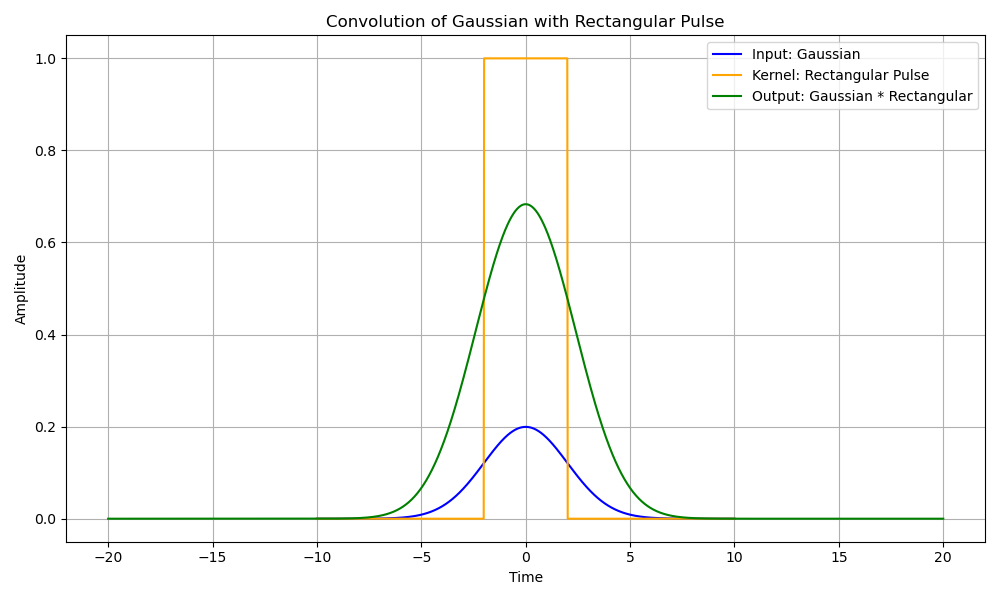
\includegraphics[width=0.6\textwidth]{figs/gaus_2.png}
    \caption{T = 2}
    \label{fig:gaus_2}
\end{figure}
\begin{figure}[h]
    \centering
    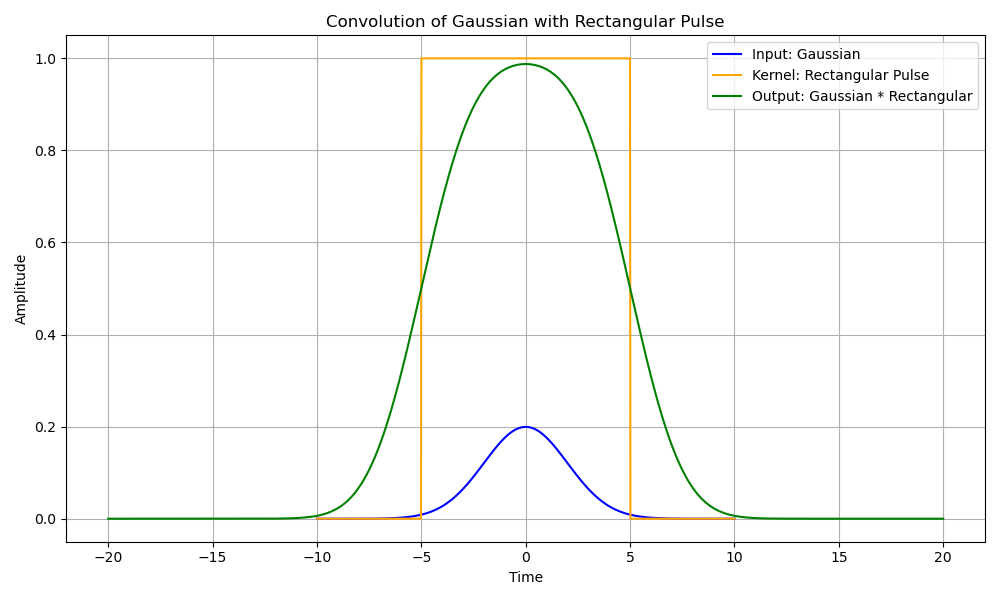
\includegraphics[width=0.6\textwidth]{figs/gaus_5.png}
    \caption{T = 5}
    \label{fig:gaus_0.5}
\end{figure}
\begin{figure}[h]
    \centering
    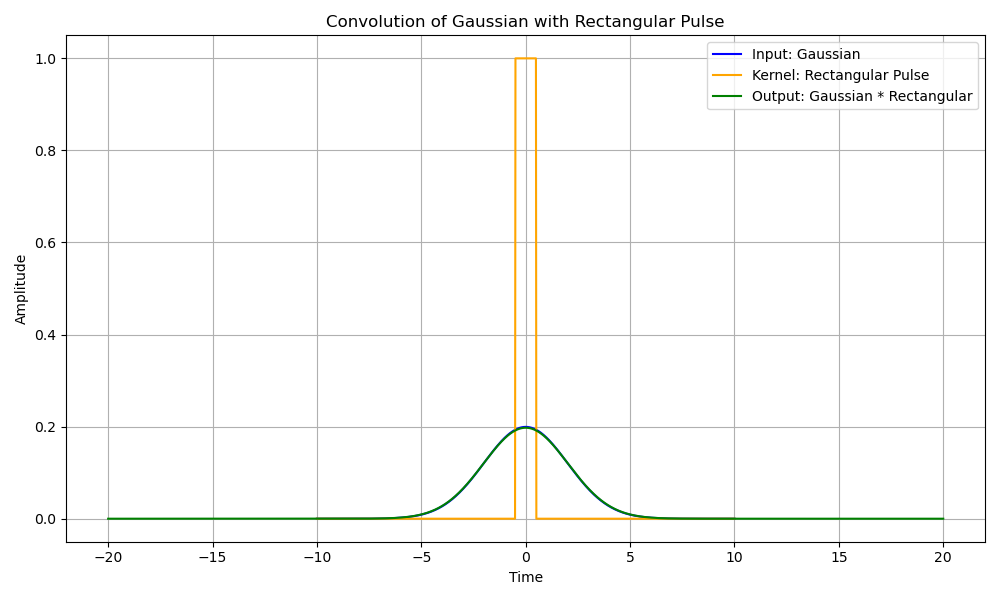
\includegraphics[width=0.6\textwidth]{figs/gaus_0.5.png}
    \caption{T = 0.5}
    \label{fig:gaus_0.5}
\end{figure}

\item In the case of Figure \ref{fig:gaus_0.5}, since the kernel itself is bell-shaped, convolving a narrow Gaussian will produce an output being very similar to the original signal, just slightly smoothed or blurred.
\item Gaussian filters are used because - \\
\begin{itemize}
\item Smooth
\item Decay to zero rapidly
\item Simple analytical formula
\item \textbf{Central Limit Theorem :} Limit of applying filters many times is some Gaussian.
\item Separable
\begin{align*}
	G_{2} (x, y) &= G_{1} (x) G_{1} (y)
\end{align*}
\end{itemize}
\end{enumerate}

\subsection{Laplacian filter}
\begin{enumerate}
\item A Laplacian filter is a second-order derivative operator that is commonly used in image processing for edge detection and enhancement.
\item It is often implemented using a convolution kernel, which is a small matrix that is slid over the image and multiplied with the surrounding pixels to produce a new pixel value.
\item The Laplacian filter, when combined with a Gaussian blur ( Laplacian of Gaussian ), can be used to detect edges in an image.
\item Image corresponding to this is given below - \\
\begin{figure}[h]
    \centering
    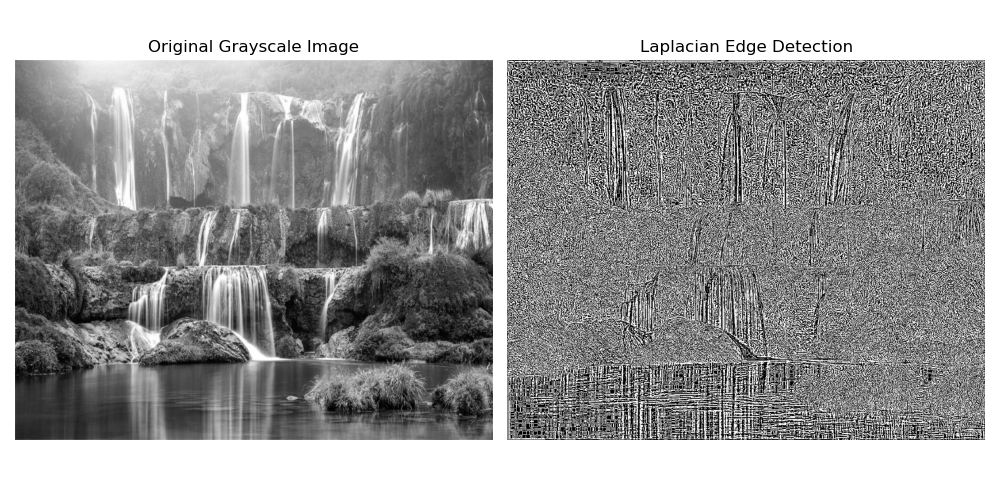
\includegraphics[width=0.6\textwidth]{figs/laplace.png}
    \caption{Edge detection using convolution}
    \label{fig:laplace}
\end{figure}
\end{enumerate}


\section{\textbf{References}}
\href{https://en.wikipedia.org/wiki/Gaussian_filter}{https://en.wikipedia.org/wiki/Gaussian_filter} \\
\href{https://www.sciencedirect.com/topics/engineering/laplacian-filter}{https://www.sciencedirect.com/topics/engineering/laplacian-filter} \\
\href{https://www.cs.princeton.edu/courses/archive/fall16/cos429/notes/cos429_f16_lecture03_filtering.pdf}{https://www.cs.princeton.edu/courses/archive/fall16/cos429/notes/cos429_f16_lecture03_filtering.pdf} \\
\href{https://people.iith.ac.in/seshadri/Courses/DETT/DETT-2025-M.html}{https://people.iith.ac.in/seshadri/Courses/DETT/DETT-2025-M.html} \\
\end{document}
